%%%%%%%%%%%%%%%%%%%%%%%%%%%%%%%%%%%%%%%%%%%%%%%%%%%%%%%%%%%%%%%%%%%%%%
% Overleaf (WriteLaTeX) Example: Molecular Chemistry Presentation
%
% Source: http://www.overleaf.com
%
% In these slides we show how Overleaf can be used with standard 
% chemistry packages to easily create professional presentations.
% 
% Feel free to distribute this example, but please keep the referral
% to overleaf.com
% 
%%%%%%%%%%%%%%%%%%%%%%%%%%%%%%%%%%%%%%%%%%%%%%%%%%%%%%%%%%%%%%%%%%%%%%

\documentclass{beamer}

\mode<presentation>
{
  \usetheme{Madrid}       % or try default, Darmstadt, Warsaw, ...
  \usecolortheme{default} % or try albatross, beaver, crane, ...
  \usefonttheme{default}    % or try default, structurebold, ...
  \setbeamertemplate{navigation symbols}{}
  \setbeamertemplate{caption}[numbered]
} 

\usepackage[english]{babel}
\usepackage[utf8x]{inputenc}
\usepackage{graphicx}
\usepackage{hyperref}
  \hypersetup{colorlinks=true}
  \hypersetup{urlcolor=blue}
  \hypersetup{linkcolor = .}
\usepackage{xcolor}
\usepackage{siunitx}
  \sisetup{separate-uncertainty = true}
\usepackage{physics}
\usepackage[font=small,labelfont=bf]{caption}
\usepackage{subcaption}
\usepackage[en-GB]{datetime2}
\usepackage{overpic}
\usepackage{feynmp}
\DeclareGraphicsRule{*}{mps}{*}{}
\usepackage{scalerel}
\newcommand{\mylbrace}[2]{\vspace{#2pt}\hspace{6pt}\scaleleftright[\dimexpr5pt+#1\dimexpr0.06pt]{\lbrace}{\rule[\dimexpr2pt-#1\dimexpr0.5pt]{-4pt}{#1pt}}{.}}
\newcommand{\myrbrace}[2]{\vspace{#2pt}\scaleleftright[\dimexpr5pt+#1\dimexpr0.06pt]{.}{\rule[\dimexpr2pt-#1\dimexpr0.5pt]{-4pt}{#1pt}}{\rbrace}\hspace{6pt}}

% Trim in percent
\usepackage{adjustbox}

% No "Figure" prefix
\setbeamertemplate{caption}{\raggedright\insertcaption\par}

% Nice decay amplitude diagrams
\usepackage{amsmath,amssymb,tikz-cd}

% Strike out text
\usepackage[normalem]{ulem}

% For figures with text overlay
\usepackage{overpic}

% Coloured text box
\usepackage[most]{tcolorbox}

% More bullet styles
\usepackage{pifont}

% Here's where the presentation starts, with the info for the title slide
\title[Charm physics]{Charm physics at BESIII}

\author[Martin Tat]{Martin Tat, on behalf of the BESIII Collaboration}
\institute[University of Oxford]{\normalsize University of Oxford\\ \vspace{0.3cm}\normalsize FPCP Conference}
\date{30th May 2023}

\titlegraphic{
\includegraphics[height = 2cm]{OxfordLogo.pdf}\hspace{1cm}~%
              
\includegraphics[height = 2cm]{bes3.jpg}}

\begin{document}

\begin{frame}
  \titlepage
\end{frame}

% These three lines create an automatically generated table of contents.
\begin{frame}{Outline}
  \tableofcontents
\end{frame}

\section{Charm physics at the BESIII experiment}
\begin{frame}{The BESIII experiment}
  \begin{itemize}
    \item{BEPCII is a symmetric $e^+e^-$ collider with a peak luminosity of $\SI{1e33}{\per\centi\meter\squared\per\second}$ at $\sqrt{s} = \SI{3.773}{\giga\eV}$}
    \item{Tracking: Helium-based multilayer drift chamber (MDC)}
    \item{PID: Plastic scintillator TOF system and $\dv{E}{x}$}
    \item{Magnet: $\SI{1.0}{\tesla}$ superconducting solenoid}
    \item{Neutral particle tracking: CsI(Tl) electromagnetic calorimeter (EMC)}
  \end{itemize}
  \begin{figure}
    \centering
    \begin{subfigure}{0.5\textwidth}
      \centering
      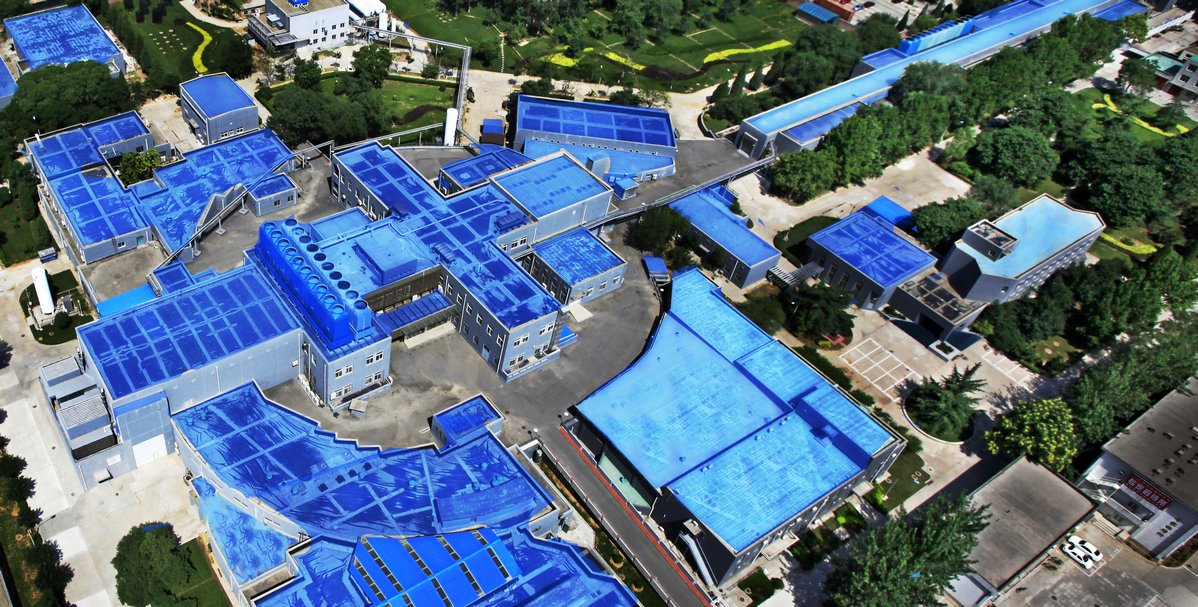
\includegraphics[width = 1.0\textwidth]{Figures/BEPCII.jpg}
    \end{subfigure}%
    \begin{subfigure}{0.5\textwidth}
      \centering
      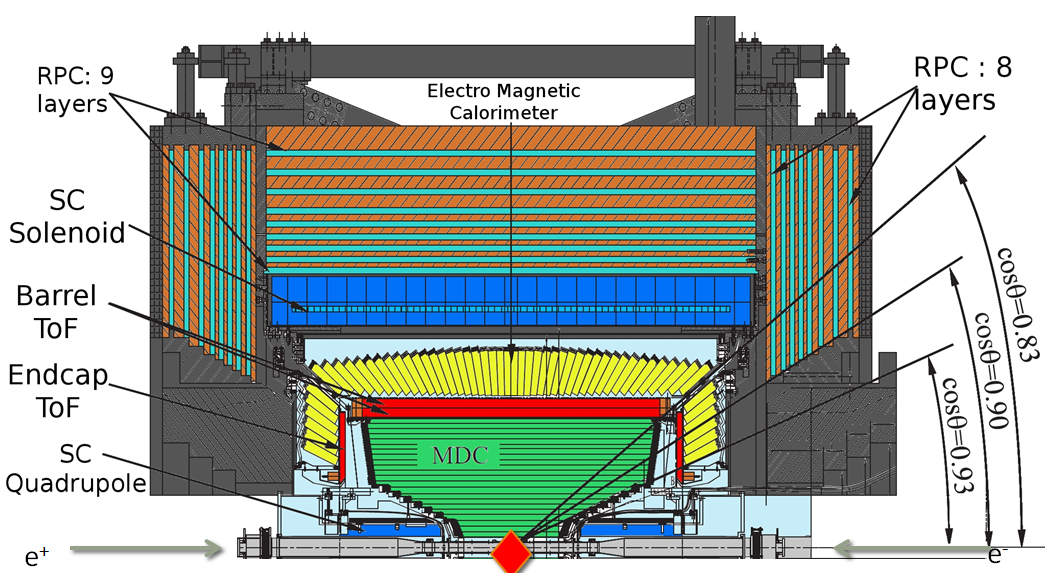
\includegraphics[width = 1.0\textwidth]{Figures/BESIII.png}
    \end{subfigure}
    \caption*{Overview of (left) BEPCII and (right) BESIII.}
  \end{figure}
\end{frame}

\begin{frame}{The BESIII experiment}
  \begin{columns}
    \begin{column}{0.5\textwidth}
      \vspace{0.0cm}
      {\large Key datasets for charm physics:}
      \begin{itemize}
      \item{2010-2011: $\SI{2.9}{\per\femto\barn}$ at $\psi(3770)$}
      \item{2013-2019: $\SI{7.3}{\per\femto\barn}$ of $D_s\bar{D_s^*}$}
      \item{2020: $\SI{4.5}{\per\femto\barn}$ of $\Lambda_c^+\bar{\Lambda_c^-}$}
      \item{2021-2022: $\SI{5.0}{\per\femto\barn}$ at $\psi(3770)$}
      \item{2022-: $\sim\SI{8}{\per\femto\barn}$ at $\psi(3770)$}
      \end{itemize}
    \end{column}
    \begin{column}{0.5\textwidth}
      \vspace{0.5cm}
      \begin{figure}
        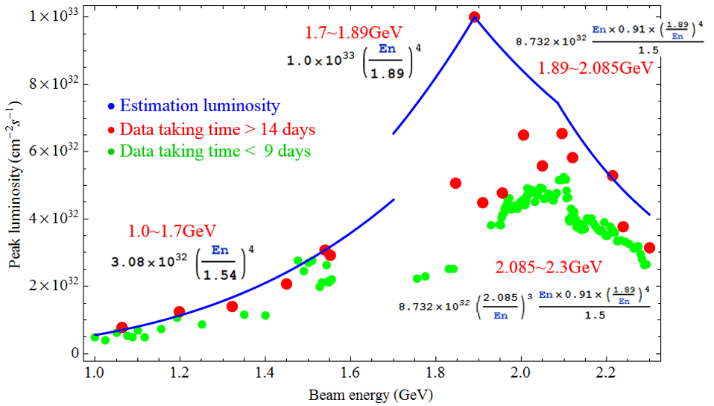
\includegraphics[width=1.0\textwidth]{Figures/BEPCII_Luminosity.png}
        \caption*{BEPCII peak luminosity.}
      \end{figure}
    \end{column}
  \end{columns}
  \begin{block}{}<all:0>
    Charm threshold data at $\psi(3770)\to D\bar{D}$ provide a unique access to strong-phase information that is essential for charm mixing and $\gamma$ measurements at $B$ factories
  \end{block}
\end{frame}

\begin{frame}{The BESIII experiment}
  \begin{columns}
    \begin{column}{0.5\textwidth}
      \vspace{0.0cm}
      {\large Key datasets for charm physics:}
      \begin{itemize}
      \item[\ding{217}]{2010-2011: $\SI{2.9}{\per\femto\barn}$ at $\psi(3770)$}
      \item{2013-2019: $\SI{7.3}{\per\femto\barn}$ of $D_s\bar{D_s^*}$}
      \item{2020: $\SI{4.5}{\per\femto\barn}$ of $\Lambda_c^+\bar{\Lambda_c^-}$}
      \item[\ding{217}]{2021-2022: $\SI{5.0}{\per\femto\barn}$ at $\psi(3770)$}
      \item[\ding{217}]{2022-: $\sim\SI{8}{\per\femto\barn}$ at $\psi(3770)$}
      \end{itemize}
    \end{column}
    \begin{column}{0.5\textwidth}
      \vspace{0.5cm}
      \begin{figure}
        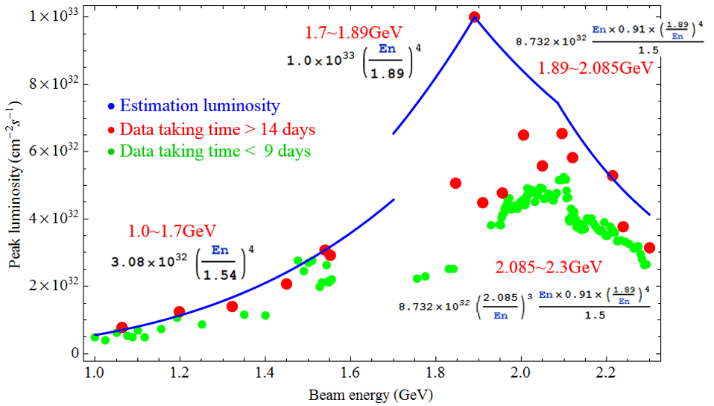
\includegraphics[width=1.0\textwidth]{Figures/BEPCII_Luminosity.png}
        \caption*{BEPCII peak luminosity.}
      \end{figure}
    \end{column}
  \end{columns}
  \begin{block}{}
    Charm threshold data at $\psi(3770)\to D\bar{D}$ provide a unique access to strong-phase information that is essential for charm mixing and $\gamma$ measurements at $B$ factories
  \end{block}
\end{frame}

\begin{frame}{Recent charm results from BESIII}
  \vspace{0.0cm}
  {\large BESIII has a rich programme of charm physics:}
  \begin{enumerate}
    \item{Strong-phase measurements}
    \begin{itemize}
      \item{Measurement of $\delta_{K\pi}$ \href{https://link.springer.com/article/10.1140/epjc/s10052-022-10872-2}{EPJC \textbf{82} 1009 (2022)}}
      \item{$D\to K^-\pi^+\pi^-\pi^+$ strong-phase measurement \href{https://link.springer.com/article/10.1007/JHEP05(2021)164}{JHEP \textbf{5} (2021) 164}}
      \item{$D\to K^+K^-\pi^+\pi^-$ $F_+$ measurement \href{https://journals.aps.org/prd/abstract/10.1103/PhysRevD.107.032009}{Phys. Rev. D \textbf{107} 032009}}
    \end{itemize}
    \item{Amplitude analysis}
    \item{Semileptonic charm decays}
    \item{Searches for rare decays}
    \item{Branching fraction measurements}
  \end{enumerate}
  \begin{center}
    {\Large No time to cover all topics in this talk!\\
      I will mainly focus on strong-phase measurements in charm decays...}
  \end{center}
\end{frame}

\begin{frame}{Recent charm results from BESIII}
  \begin{enumerate}
    \item{Strong-phase measurements}
    \begin{itemize}
      \item{$D\to K_S^0\pi^+\pi^-\pi^0$ $F_+$ measurement \href{https://arxiv.org/abs/2305.03975}{arXiv:2305.03975}}
    \end{itemize}
    \item{Amplitude analysis}
    \begin{itemize}
      \item{Amplitude analysis of $D^0\to K_L^0\pi^+\pi^-$ \href{https://arxiv.org/abs/2212.09048}{arXiv:2212.0904}}
      \item{Observation of an $a_0(980)$-like state \href{https://journals.aps.org/prl/abstract/10.1103/PhysRevLett.129.182001}{Phys. Rev. Lett. \textbf{129}, 182001}}
    \end{itemize}
    \item{Semileptonic charm decays}
    \begin{itemize}
      \item{First study of $D_s^{*+}\to e^+\nu_e$ \href{https://arxiv.org/abs/2304.12159}{arXiv:2304.12159}}
      \item{$D_s^+\to\tau^+\nu_\tau$ \href{https://arxiv.org/abs/2303.12600}{arXiv:2303.12600}, \href{https://arxiv.org/abs/2303.12600}{arXiv:2303.12600}, \href{https://arxiv.org/abs/2303.12468}{arXiv:2303.12468}}
      \item{Study of $D_s^+\to\pi^+\pi^-e^+\nu_e$ \href{https://arxiv.org/abs/2303.12927}{arXiv:2303.12927}}
    \end{itemize}
    \item{Searches for rare decays}
    \begin{itemize}
      \item{See \href{https://indico.cern.ch/event/1166059/contributions/5305453/}{Liang's talk}}
    \end{itemize}
  \end{enumerate}
  \begin{center}
    {\Large ... but here I provide references to some recent interesting charm results}
  \end{center}
\end{frame}

\begin{frame}{Double-tag analysis}
  \begin{figure}[H]
    \begin{fmffile}{fgraph/fgraph_flavour_decays}
      \setlength{\unitlength}{1cm}
      \begin{fmfgraph*}(8,4)
        \fmfstraight
        \fmfleft{i4,i3,i2,i1}
        \fmfright{g1,o1,o2,g2}
        \fmflabel{$K^-$}{o1}
        \fmflabel{$K^+$}{o2}
        \fmflabel{$K^-$}{i1}
        \fmflabel{$\pi^+$}{i2}
        \fmflabel{$\pi^-$}{i3}
        \fmflabel{$\pi^+$}{i4}
        \fmf{plain}{wL,i1}
        \fmf{plain}{wL,i2}
        \fmf{plain}{wL,i3}
        \fmf{plain}{wL,i4}
        \fmf{plain}{wR,o1}
        \fmf{plain}{wR,o2}
        \fmf{phantom}{wR,g1}
        \fmf{phantom}{wR,g2}
        \fmf{dashes,tension=10.0}{wR,w}
        \fmf{dashes,tension=10.0}{wL,w}
        \fmfv{decor.shape=circle,decor.filled=shaded,decor.size=0.4cm,label=$D^0$,label.angle=90,label.dist=0.4cm}{wR}
        \fmfv{decor.shape=circle,decor.filled=shaded,decor.size=0.4cm,label=$\bar{D^0}$,label.angle=90,label.dist=0.4cm}{wL}
        \fmfblob{0.5cm}{wL}
        \fmfv{decor.shape=hexagram,decor.filled=empty,decor.size=0.3cm,label=$\psi(3770)$,label.angle=-90,label.dist=0.4cm}{w}
      \end{fmfgraph*}
    \end{fmffile}
    \vspace{0.5cm}
    \caption*{Double-tag method}
  \end{figure}
  \begin{center}
    The $D$ mesons are produced in a quantum correlated state:\\
    $\lvert\psi\rangle = \frac{1}{\sqrt{2}}\big(\lvert D^0\rangle\lvert\bar{D^0}\rangle - \lvert\bar{D^0}\rangle\lvert D^0\rangle\big)$
  \end{center}
\end{frame}

\begin{frame}{Double-tag analysis}
  \begin{figure}[H]
    \begin{fmffile}{fgraph/fgraph_CP_decays}
      \setlength{\unitlength}{1cm}
      \begin{fmfgraph*}(8,4)
        \fmfstraight
        \fmfleft{i4,i3,i2,i1}
        \fmfright{g1,o1,o2,g2}
        \fmflabel{$K^-$}{o1}
        \fmflabel{$K^+$}{o2}
        \fmflabel{$K^-$}{i1}
        \fmflabel{$\pi^+$}{i2}
        \fmflabel{$\pi^-$}{i3}
        \fmflabel{$\pi^+$}{i4}
        \fmf{plain}{wL,i1}
        \fmf{plain}{wL,i2}
        \fmf{plain}{wL,i3}
        \fmf{plain}{wL,i4}
        \fmf{plain}{wR,o1}
        \fmf{plain}{wR,o2}
        \fmf{phantom}{wR,g1}
        \fmf{phantom}{wR,g2}
        \fmf{dashes,tension=10.0}{wR,w}
        \fmf{dashes,tension=10.0}{wL,w}
        \fmfv{decor.shape=circle,decor.filled=shaded,decor.size=0.4cm,label=$D_+$,label.angle=90,label.dist=0.4cm}{wR}
        \fmfv{decor.shape=circle,decor.filled=shaded,decor.size=0.4cm,label=$D_-$,label.angle=90,label.dist=0.4cm}{wL}
        \fmfblob{0.5cm}{wL}
        \fmfv{decor.shape=hexagram,decor.filled=empty,decor.size=0.3cm,label=$\psi(3770)$,label.angle=-90,label.dist=0.4cm}{w}
      \end{fmfgraph*}
    \end{fmffile}
    \vspace{0.5cm}
    \caption*{Double-tag method}
  \end{figure}
  \begin{center}
    Equivalently, we can consider the CP even (odd) eigenstates $D_+$ ($D_-$):\\
    $\lvert\psi\rangle = \frac{1}{\sqrt{2}}\big(\lvert D_+\rangle\lvert D_-\rangle - \lvert D_-\rangle\lvert D_+\rangle\big)$
  \end{center}
\end{frame}

\begin{frame}{Double-tag analysis}
  \vspace{0.0cm}
  {\large Double-tag analysis has many advantages:}
  \begin{enumerate}
    \setlength{\itemsep}{1.0em}
    \item{$D\bar{D}$ pairs are quantum correlated, which provide direct access to the $D^0$-$\bar{D^0}$ strong-phase difference}
    \item{Measurements are, to first order, free from systematic uncertainties due to efficiencies and branching fractions}
    \item{Full reconstruction ensures that the environment is extremely clean}
  \end{enumerate}
  \vspace{1.0cm}
  {\large Only one minor drawback:}
  \begin{enumerate}
    \item{Lower statistics}
  \end{enumerate}
\end{frame}

\section{\texorpdfstring{$D\to K^-\pi^+$}{D2Kpi}}
\begin{frame}{$D\to K^-\pi^+$}
\begin{tcolorbox}[enhanced,frame style image=blueshade_cropped.png,
  opacityback=0.75,opacitybacktitle=0.25,
  colback=blue!5!white,colframe=blue!75!black,
  title=\color{white}{\href{https://link.springer.com/article/10.1140/epjc/s10052-022-10872-2}{\color{white}{EPJC \textbf{82} 1009 (2022)}}}]
  {\Large Improved measurement of the strong-phase difference $\delta_D^{K\pi}$ in quantum-correlated $D\bar{D}$ decays}
\end{tcolorbox}
  What is measured:
  \begin{itemize}
    \item{Strong-phase difference between CF and DCS $D\to K^\mp\pi^\pm$ decays}
  \end{itemize}
  Analysis strategy:
  \begin{itemize}
    \item{Large boost in statistics by including $D\to K_L^0X$ tags}
    \item{Independent determinations of $D\to K_L^0X$ branching fractions}
  \end{itemize}
  Significance:
  \begin{itemize}
    \item{Most precise measurement of $\delta_D^{K\pi}$ in quantum-correlated $D\bar{D}$ decays}
  \end{itemize}
\end{frame}

\begin{frame}{$D\to K^-\pi^+$}
  \vspace{0.0cm}
  {\large The strong-phase difference $\delta_D^{K\pi}$ between CF and DCS $D\to K^-\pi^+$ is a key parameter in charm physics:}
  \begin{center}
    $r_D^{K\pi}\exp\big(-i\delta_D^{K\pi}) = \frac{\langle K^+\pi^-\lvert D^0\rangle}{\langle K^+\pi^-\lvert \bar{D^0}\rangle}$
  \end{center}
  \vspace{0.5cm}
  {\large Analysis is split into three main sections:}
  \vspace{0.2cm}
  \begin{enumerate}
    \setlength{\itemsep}{1.0em}
    \item{Determination of $D\to K_L^0X$ branching fractions}
    \item{Measurement of the asymmetry $\mathcal{A}_{K\pi}$ using $C\!P$ tags}
    \item{Measurement of $r_D^{K\pi}\cos(\delta_D^{K\pi})$ and $r_D^{K\pi}\sin(\delta_D^{K\pi})$ with $K_{S, L}^0\pi^+\pi^-$ tags}
  \end{enumerate}
\end{frame}

\begin{frame}{$D\to K^-\pi^+$}
  \begin{itemize}
    \item{Branching fractions must be determined independently of $D\to K^-\pi^+\implies$ Measure using pure $C\!P$ tags}
    \item{$K_L^0\pi^0$ and $K_L^0\omega$ are $C\!P$-even decays, and must therefore be tagged by $C\!P$-odd decays}
    \begin{itemize}
      \item{$K_S^0\pi^0$, $K_S^0\eta$, $K_S^0\eta'(\pi^+\pi^-\eta, \pi^+\pi^-\gamma)$, $K_S^0\omega$}
    \end{itemize}
  \end{itemize}
  \begin{figure}
    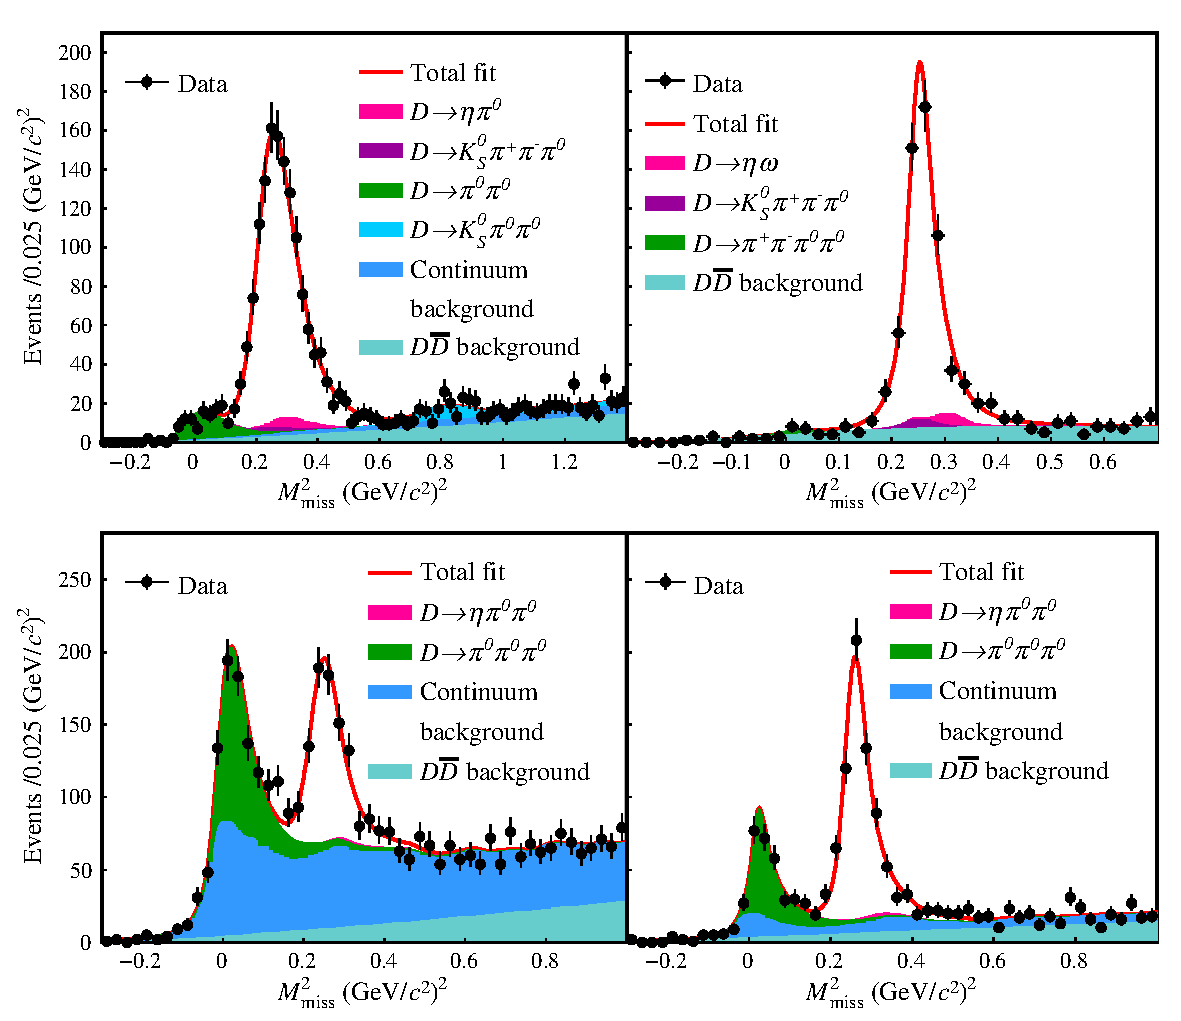
\includegraphics[height=4.5cm,trim={0 8.5cm 0 0},clip=true]{Figures/Delta_Kpi_KLX_DT_Fits.pdf}
    \caption*{Missing mass squared in $C\!P$-tagged (left) $D\to K_L^0\pi^0$ and (right) $D\to K_L^0\omega$.}
  \end{figure}
\end{frame}

\begin{frame}{$D\to K^-\pi^+$}
  \begin{itemize}
    \item{Branching fractions must be determined independently of $D\to K^-\pi^+\implies$ Measure using pure $C\!P$ tags}
    \item{Similarly, $K_L^0\pi^0\pi^0$ is a $C\!P$-odd decay and is tagged by $C\!P$-even decays}
    \begin{itemize}
      \item{$K^+K^-$, $\pi^+\pi^-$, $K_S^0\pi^0\pi^0$, $\pi^+\pi^-\pi^0$}
    \end{itemize}
  \end{itemize}
  \begin{figure}
    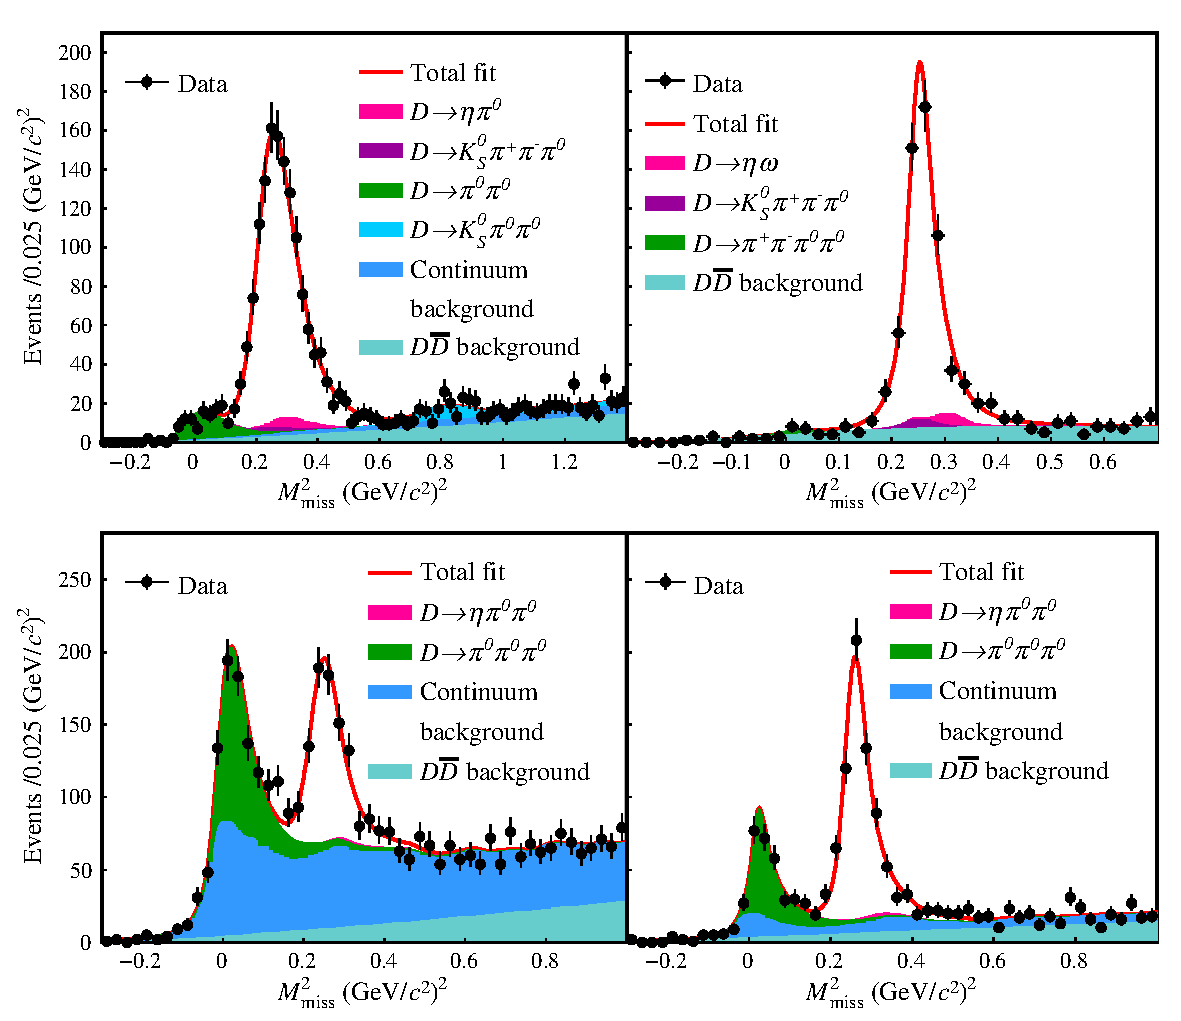
\includegraphics[height=4.5cm,trim={0 0 0 8.8cm},clip=true]{Figures/Delta_Kpi_KLX_DT_Fits.pdf}
    \caption*{Missing mass squared in (left) $\pi^+\pi^-\pi^0$ tags and all other tags (left).}
  \end{figure}
\end{frame}

\begin{frame}{$D\to K^-\pi^+$}
  \vspace{0.0cm}
  {\large Asymmetry $\mathcal{A}_{K\pi}$ of the branching fraction, tagged with $C\!P$-even and $C\!P$-odd decays, is sensitive to $\delta_D^{K\pi}$:}
  \begin{center}
    $\mathcal{A}_{K\pi} = \frac{-2r_D^{K\pi}\cos(\delta_{K\pi}) + y}{1 + (r_D^{K\pi})^2}$
  \end{center}
  Using external inputs for $y$ and $r_D^{K\pi}$, $r_D^{K\pi}\cos(\delta_D^{K\pi})$ is calculated from $\mathcal{A}_{K\pi}$
  \begin{figure}
    \centering
    \begin{subfigure}{0.5\textwidth}
      \centering
      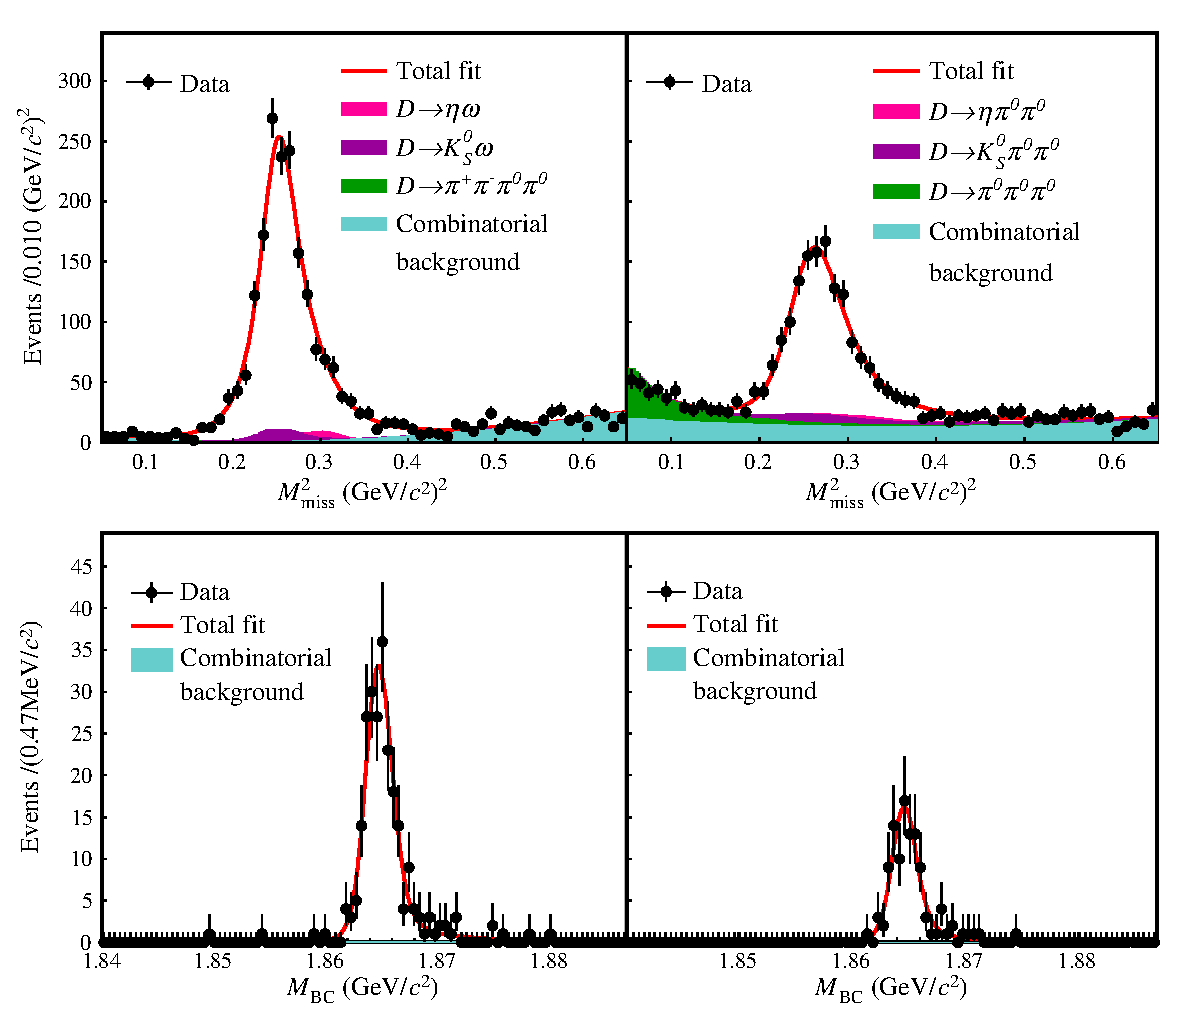
\includegraphics[height=4.0cm,trim={0 8.6cm 9.4cm 0},clip=true]{Figures/Delta_Kpi_DT_Fits.pdf}
    \end{subfigure}%
    \begin{subfigure}{0.5\textwidth}
      \centering
      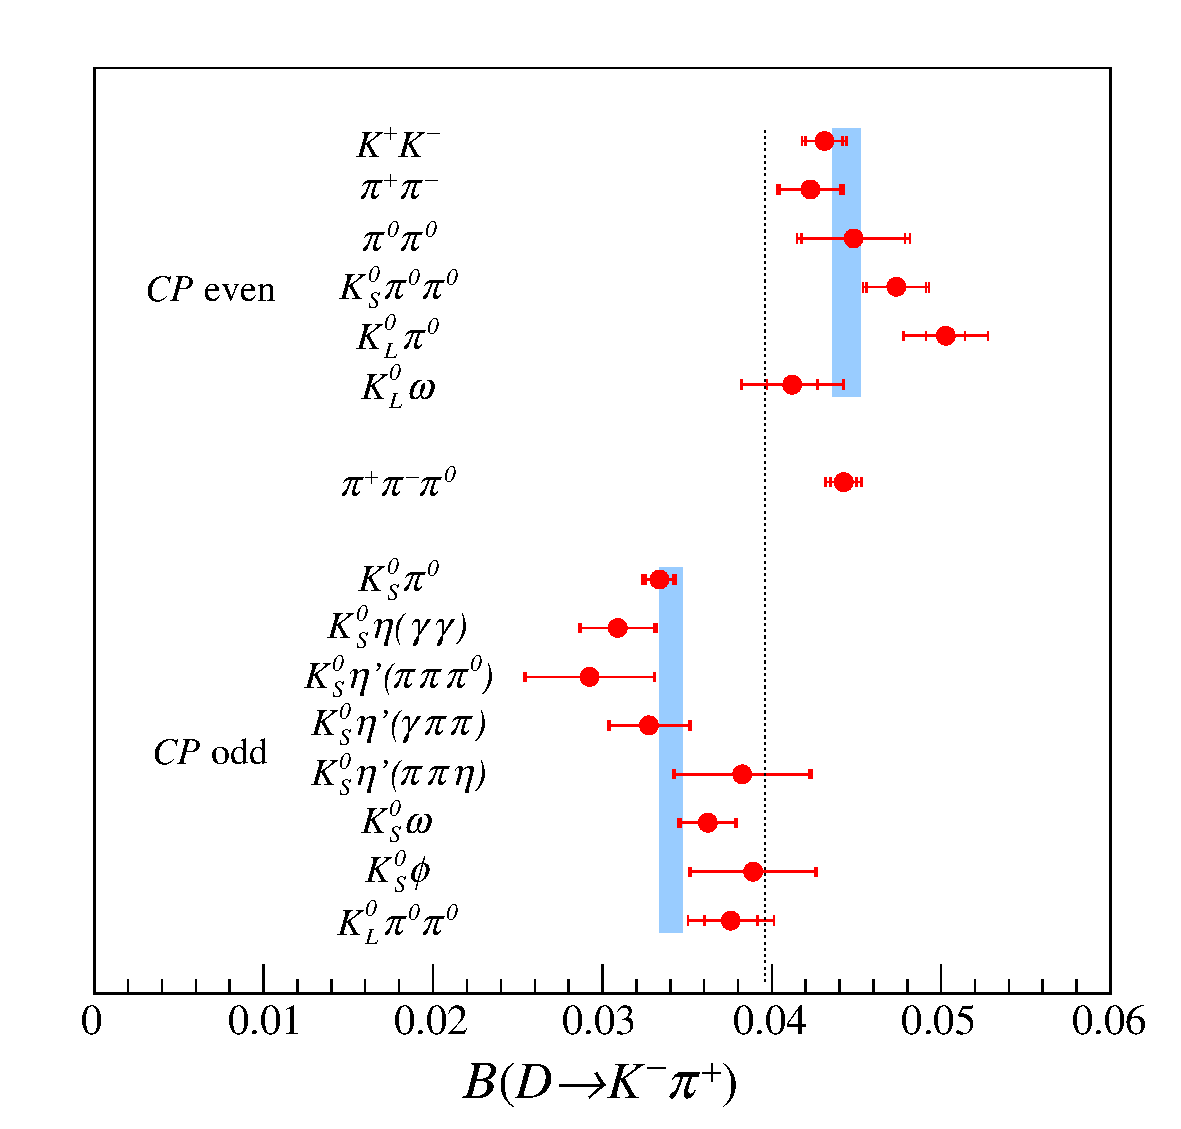
\includegraphics[height=4.0cm]{Figures/Delta_Kpi_Asymmetry.pdf}
    \end{subfigure}
    \caption*{Left: Fit of the $K^-\pi^+$ vs $K_L^0\omega$ double-tag yield. Right: Branching fraction of $D\to K^-\pi^+$ measured using $C\!P$ tags.}
  \end{figure}
\end{frame}

\begin{frame}{$D\to K^-\pi^+$}
  \vspace{0.0cm}
  {\large Double-tag yields using the $K_{S, L}^0\pi^+\pi^-$ tags, in bins of phase space, are also sensitive to $\delta_D^{K\pi}$:}
  \begin{equation*}
    Y_i\propto\Big(K_i + (r_D^{K\pi})^2K_{-i} - 2r_D^{K\pi}\sqrt{K_iK_{-i}}\Big[c_i\cos(\delta_D^{K\pi}) - s_i\sin(\delta_D^{K\pi})\Big]\Big)
  \end{equation*}
  \vspace{-0.7cm}
  \begin{columns}
    \begin{column}{0.5\textwidth}
      \begin{itemize}
      \setlength{\itemsep}{1.0em}
      \item{$\delta_D^{K\pi}$ is close to $\pi\implies$ $\sin(\delta_D^{K\pi})$ is much more sensitive to $\delta_D^{K\pi}$}
      \item{Unique determination of $\delta_D^{K\pi}$ without ambiguity}
      \item{External inputs for $K_i$, $c_i$ and $s_i$ are recalculated without inputs from $D\to K^-\pi^+$}
      \end{itemize}
    \end{column}
    \begin{column}{0.5\textwidth}
      \begin{figure}
        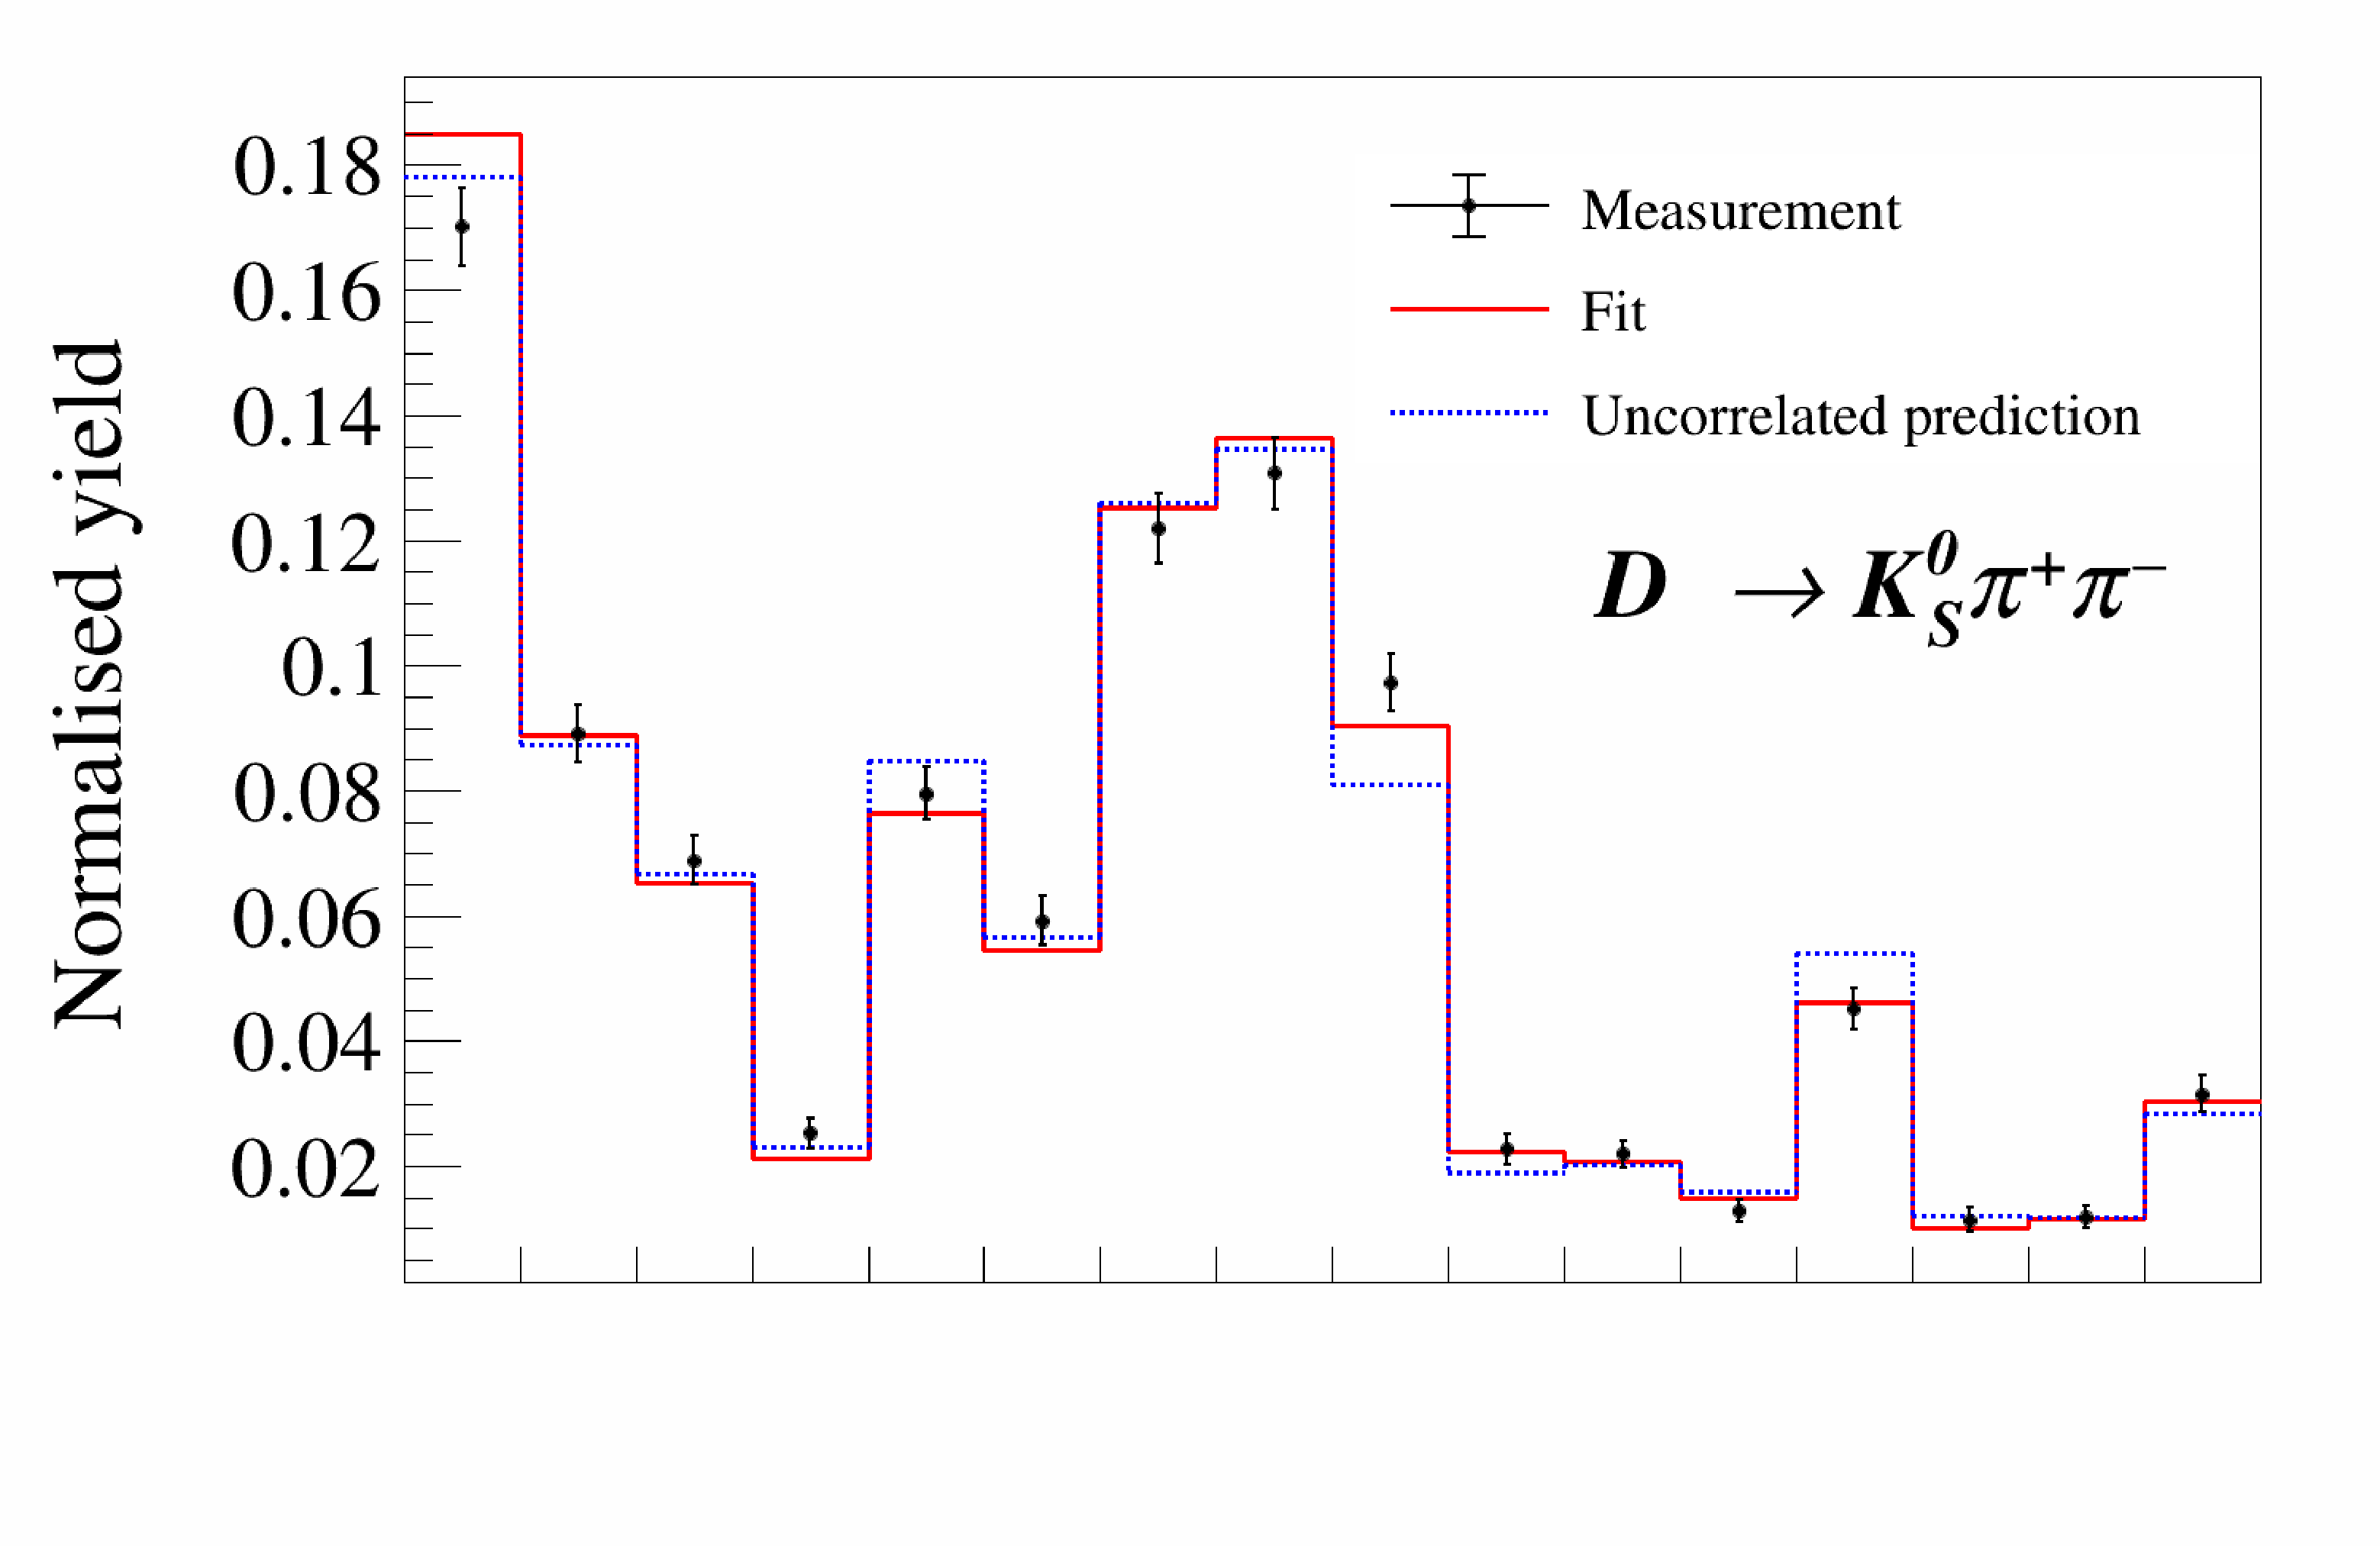
\includegraphics[width=0.75\textwidth,trim={0 5.8cm 0 0},clip=true]{Figures/KSpipiVersusKpiYields.pdf}
        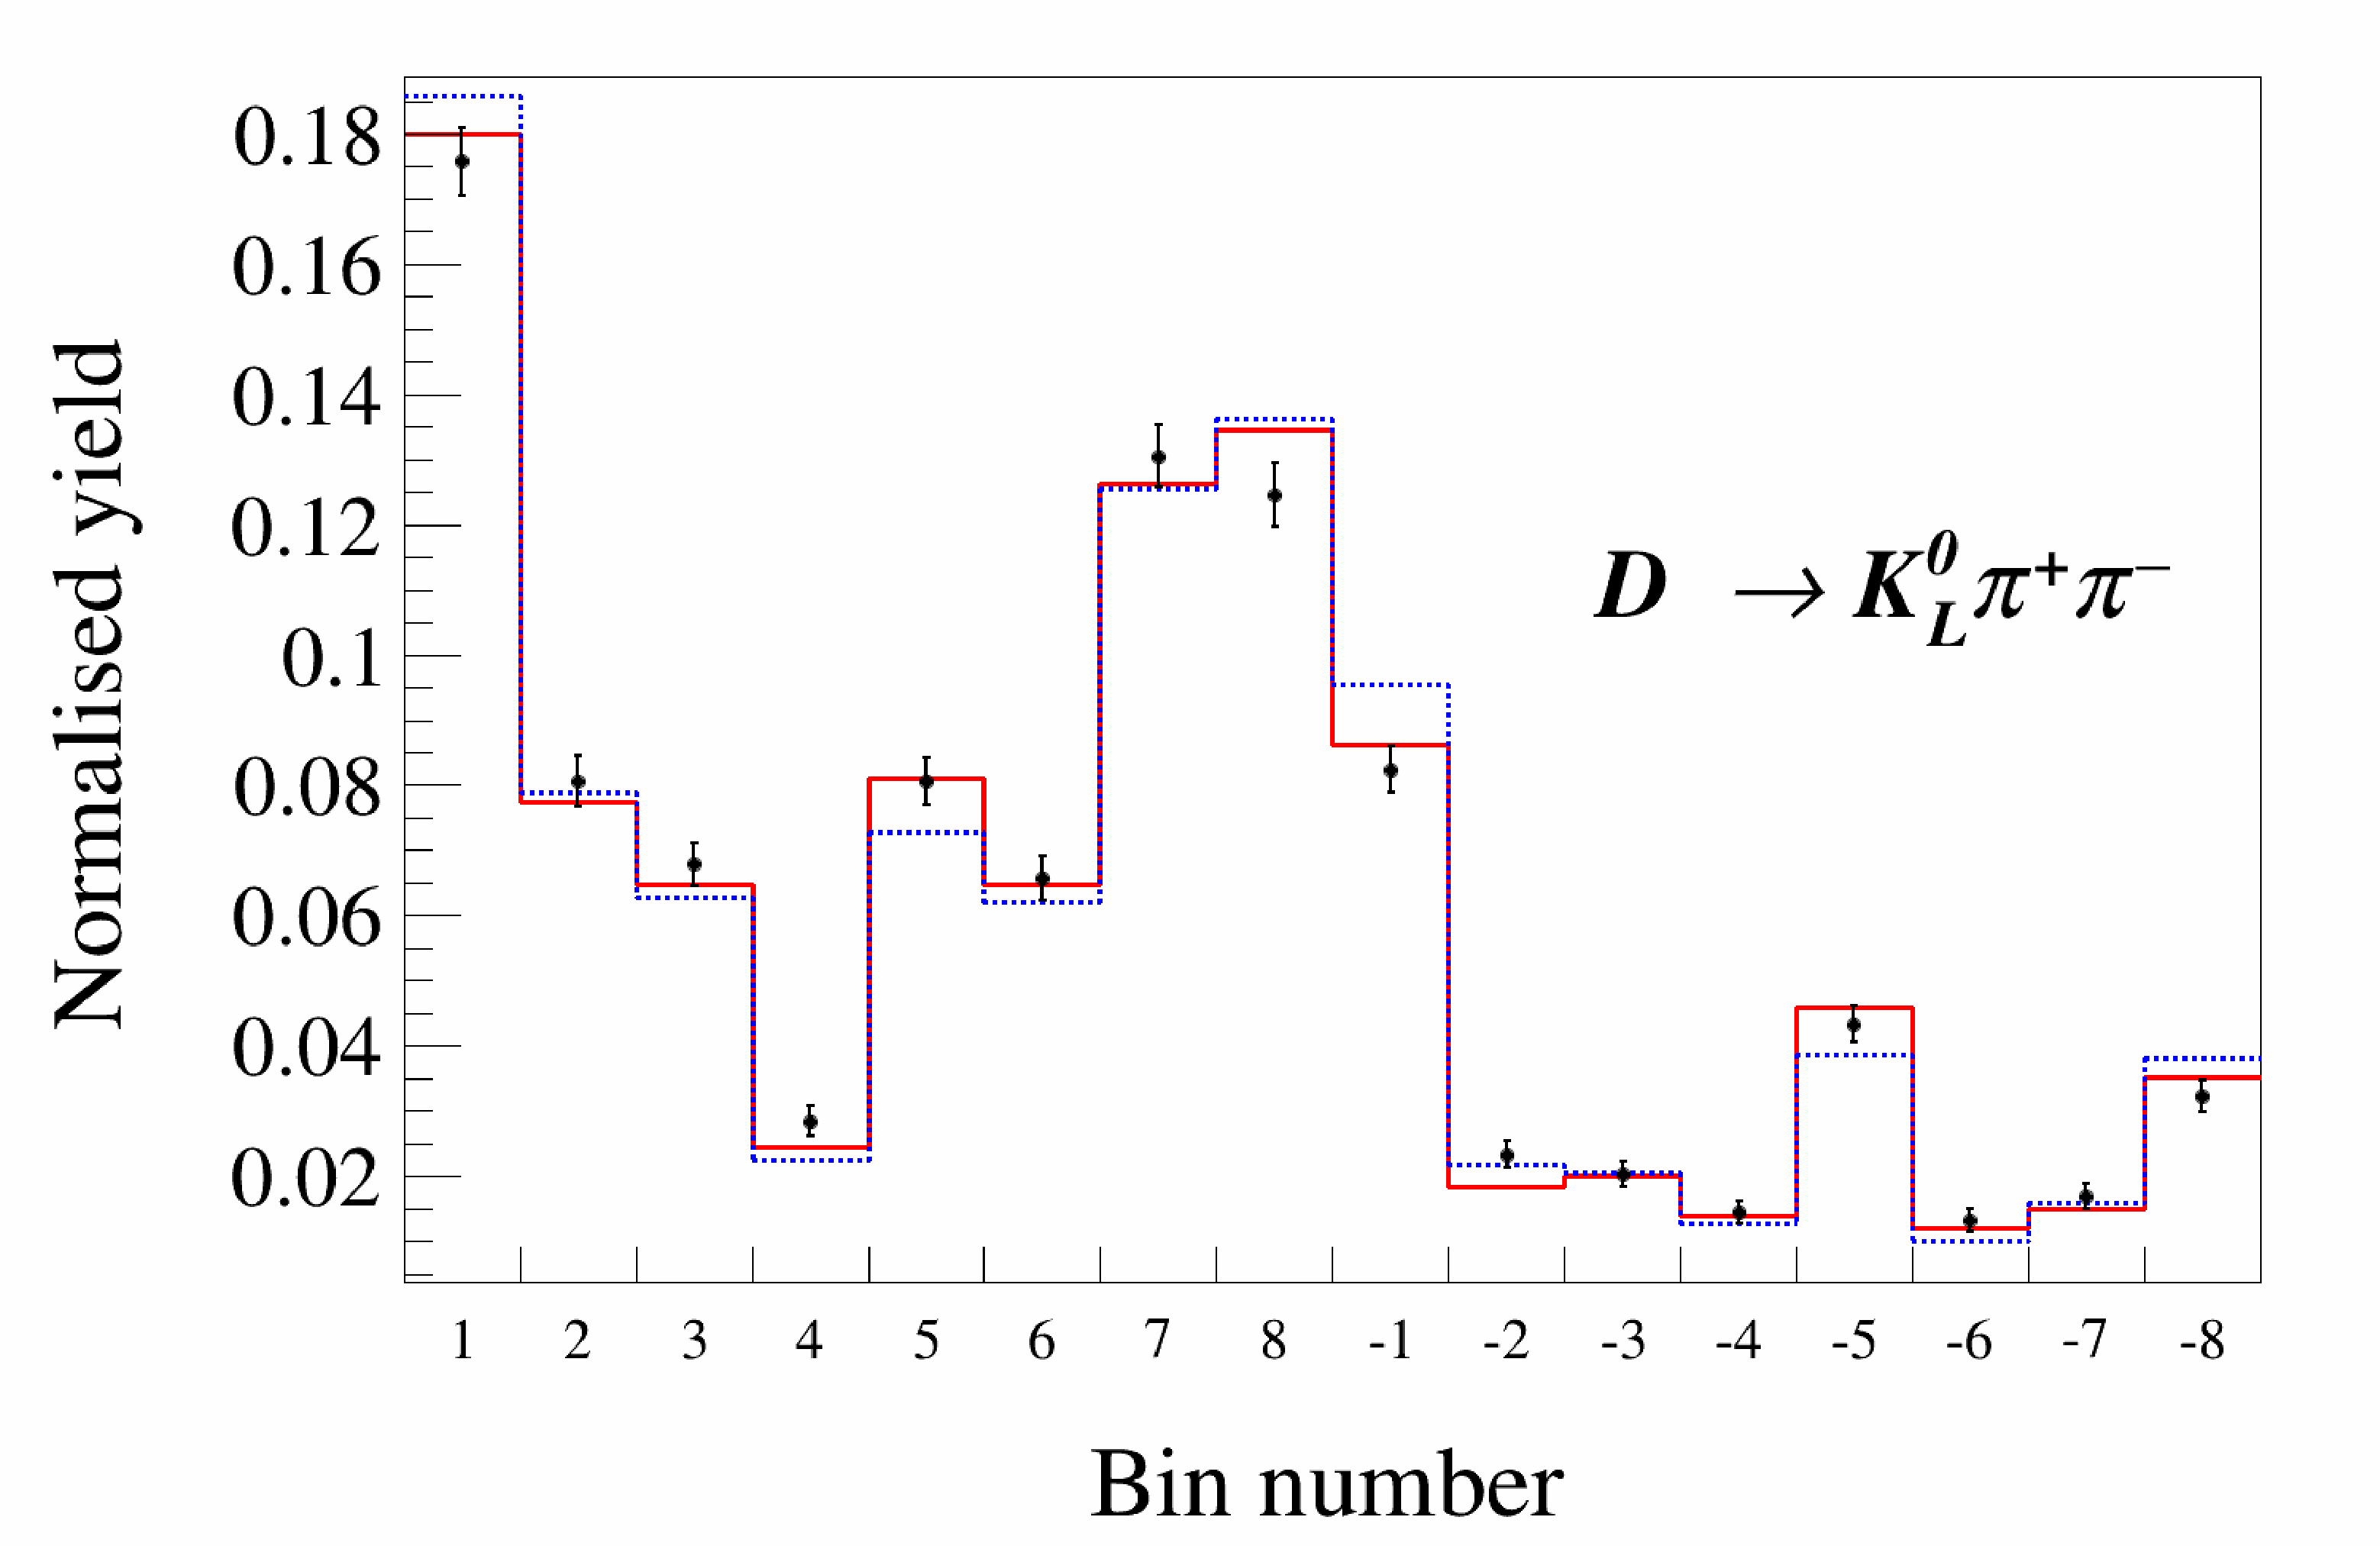
\includegraphics[width=0.75\textwidth,trim={0 0 0 2.0cm},clip=true]{Figures/KLpipiVersusKpiYields.pdf}
        \caption*{Bin yields of $D\to K_{S, L}^0\pi^+\pi^-$}
      \end{figure}
    \end{column}
  \end{columns}  
\end{frame}

\begin{frame}{$D\to K^-\pi^+$}
  \vspace{0.0cm}
  {\large Putting this all together:}
  \begin{align*}
    \delta_D^{K\pi} = (187.6^{+8.9+5.4}_{-9.7-6.4})^\circ \\
  \end{align*}
  {\large Furthermore, the following braching fractions will be valuable additions to the PDG:}
  \begin{align*}
    \mathcal{B}(D^0\to K_L^0\pi^0) =& (0.97 \pm 0.03 \pm 0.02)\times10^{-2} \\
    \mathcal{B}(D^0\to K_L^0\omega) =& (1.09 \pm 0.06 \pm 0.03)\times10^{-2} \\
    \mathcal{B}(D^0\to K_L^0\pi^0\pi^0) =& (1.26 \pm 0.05 \pm 0.03)\times10^{-2}
  \end{align*}
\end{frame}

\section{\texorpdfstring{$D\to K^-\pi^+\pi^-\pi^+$}{D2Kpipipi}}
\begin{frame}{$D\to K^-\pi^+\pi^-\pi^+$}
\begin{tcolorbox}[enhanced,frame style image=blueshade_cropped.png,
  opacityback=0.75,opacitybacktitle=0.25,
  colback=blue!5!white,colframe=blue!75!black,
  title=\color{white}{\href{https://link.springer.com/article/10.1007/JHEP05(2021)164}{\color{white}{JHEP \textbf{5} (2021) 164}}}]
  {\Large Measurement of the $D\to K^-\pi^+\pi^-\pi^-$ and $D\to K^-\pi^+\pi^0$ coherence factors and average strong-phase differences in quantum-correlated $D\bar{D}$ decays}
\end{tcolorbox}
  What is measured:
  \begin{itemize}
    \item{Strong-phase difference and coherence factors between CF and DCS $D\to K^\mp\pi^\pm\pi^\mp\pi^\pm$ decays in phase space bins}
    \item{Phase-space integrated analysis of $D\to K^\mp\pi^\pm\pi^0$}
  \end{itemize}
  Analysis strategy:
  \begin{itemize}
    \item{Binning of 5D phase space enhances the coherence factors}
  \end{itemize}
  Significance:
  \begin{itemize}
    \item{Crucial input to one of the most precise measurements of $\gamma$}
  \end{itemize}
\end{frame}

\begin{frame}{$D\to K^-\pi^+\pi^-\pi^+$}
  \vspace{0.0cm}
  {\large The average strong-phase difference of multi-body decays may be determined analogously using $C\!P$ and multi-body tags}
  \begin{figure}
    \centering
    \begin{subfigure}{0.4\textwidth}
      \centering
      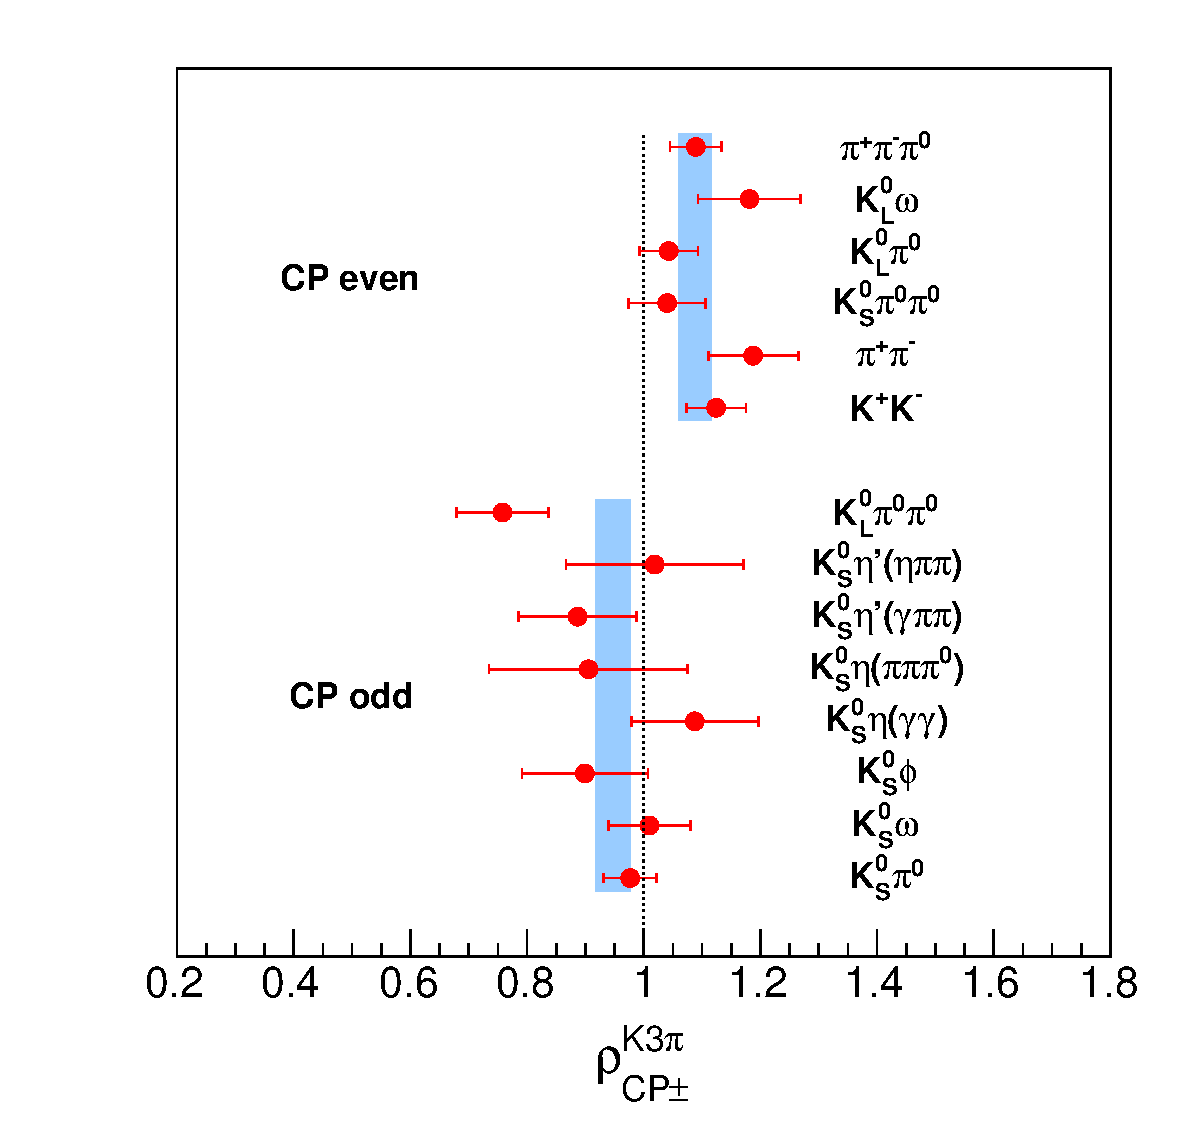
\includegraphics[height=5.0cm]{Figures/K3pi_CP_Asymmetry.pdf}
    \end{subfigure}%
    \begin{subfigure}{0.6\textwidth}
      \centering
      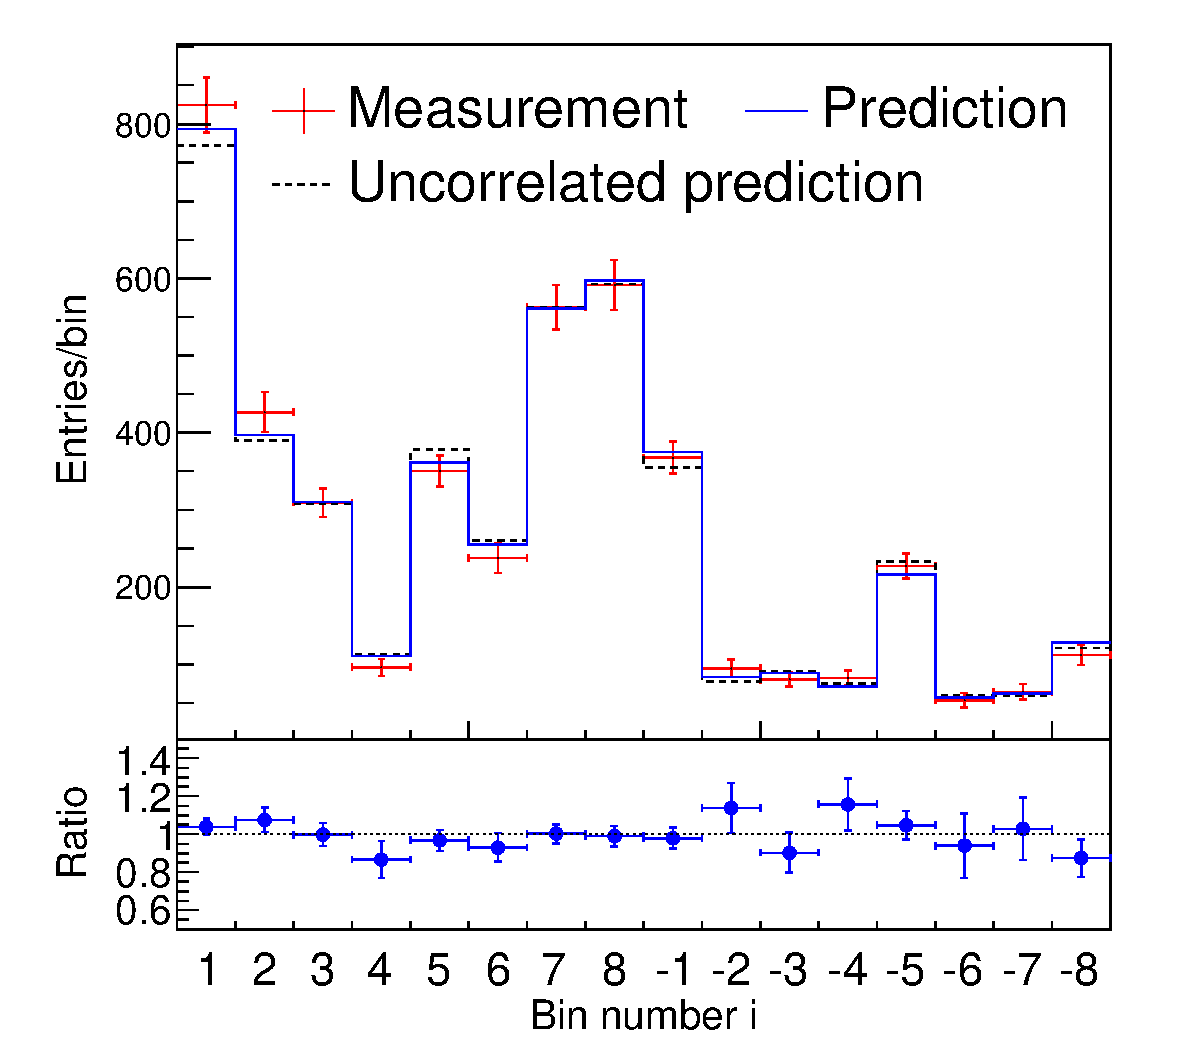
\includegraphics[height=5.0cm]{Figures/K3pi_KSpipi_yields.pdf}
    \end{subfigure}
    \caption*{Left: Asymmetry of $D\to K^-\pi^+\pi^-\pi^+$ branching fraction with $C\!P$-even and $C\!P$-odd tags. Right: Double-tag yields of $K_S^0\pi^+\pi^-$ vs $K^-\pi^+\pi^-\pi^+$.}
  \end{figure}
\end{frame}

\begin{frame}{$D\to K^-\pi^+\pi^-\pi^+$}
  \vspace{0.0cm}
  {\large However, averaging over phase space dilutes interference effects, which is parameterised in terms of the coherence factor:}
  \begin{equation*}
    R_{K3\pi}\exp(i\delta_{K3\pi})\equiv\frac{\int\dd{\vec{x}}\mathcal{A}_{\bar{D^0}\to K^+\pi^-\pi^+\pi^-}(\vec{x})\mathcal{A}^*_{D^0\to K^+\pi^-\pi^+\pi^-}(\vec{x})}{A_{\bar{D^0}\to K^+\pi^-\pi^+\pi^-}A_{D^0\to K^+\pi^-\pi^+\pi^-}}
  \end{equation*}
  \begin{figure}
    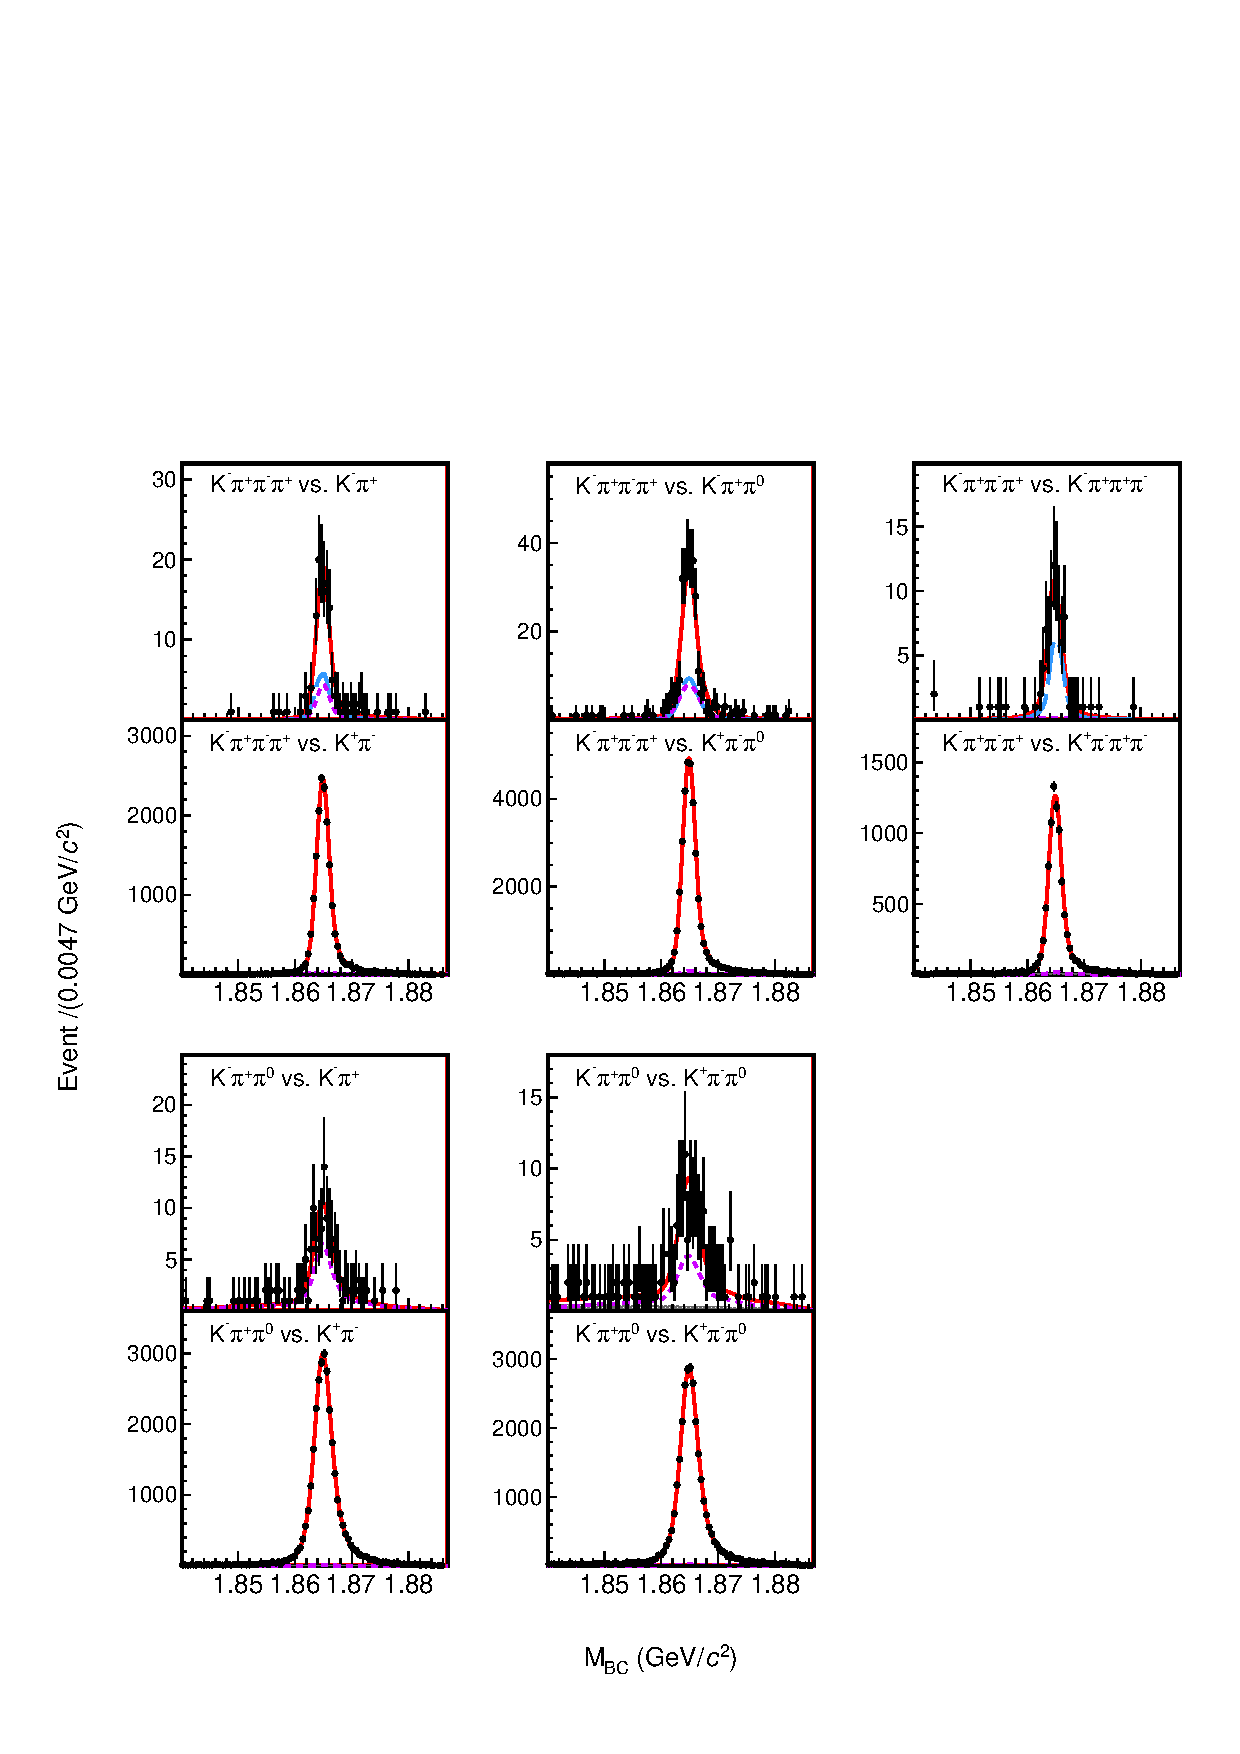
\includegraphics[height=4.5cm,trim={1.5cm 11.7cm 0 0},clip=true]{Figures/K3pi_Self_Tag.pdf}
    \caption*{Like-sign yields are proportional to $(1 - R^2)$ and brings sensitivity to $R_{K3\pi}$.}
  \end{figure}
\end{frame}

\begin{frame}{$D\to K^-\pi^+\pi^-\pi^+$}
  \vspace{0.0cm}
  {\large Fit $R_{K3\pi}$ and $\delta_{K3\pi}$: Huge improvements from CLEO-c analysis}
  \vspace{-0.2cm}
  \begin{figure}
    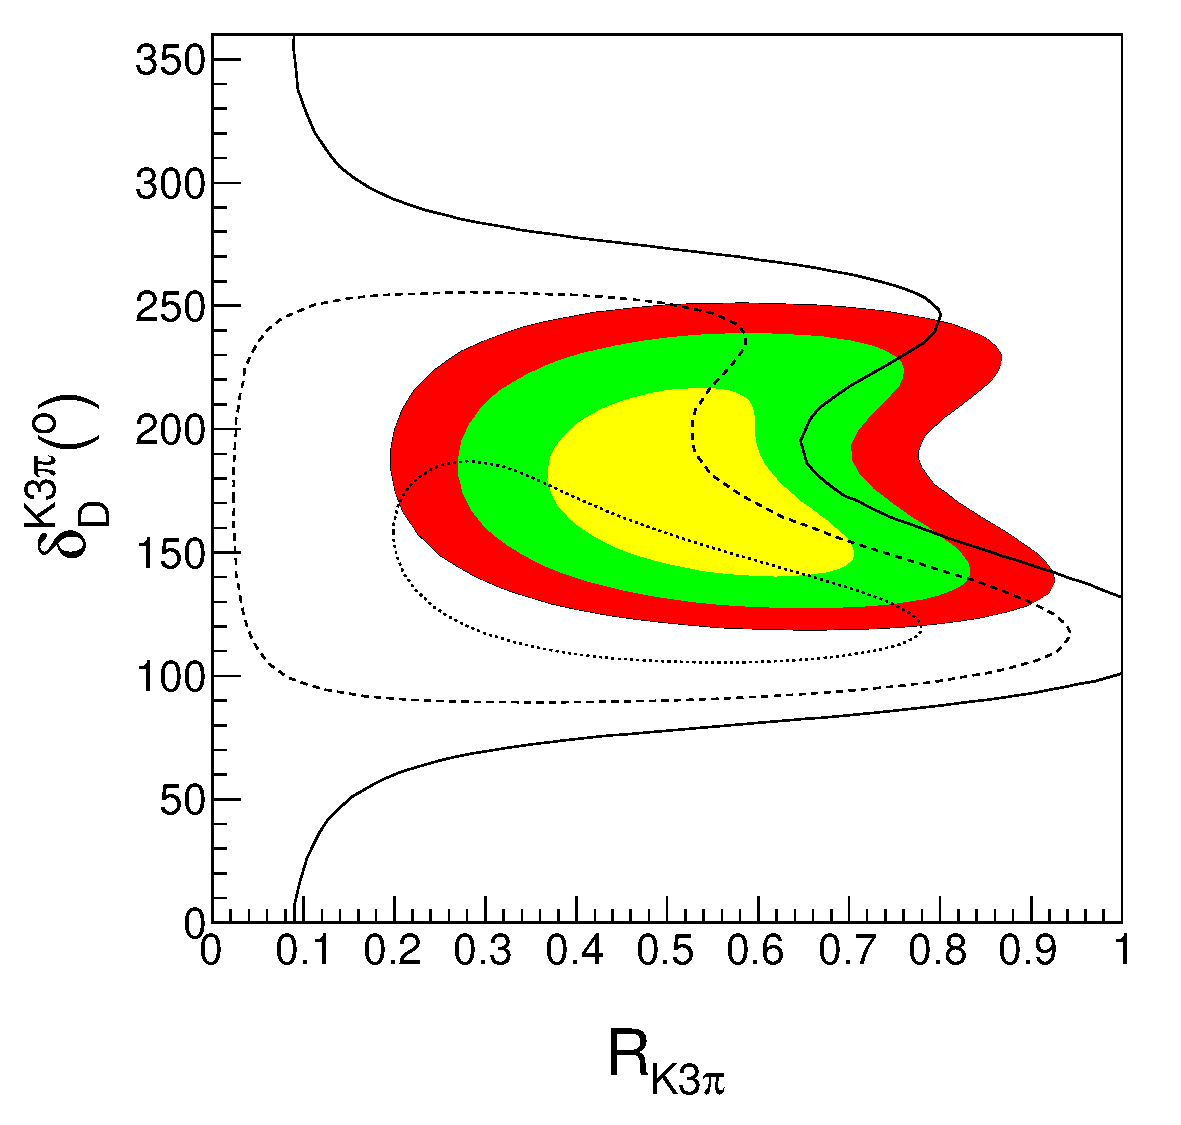
\includegraphics[width=0.5\textwidth]{Figures/K3pi_Global_Fit.pdf}
  \end{figure}
  \vspace{-0.5cm}
  {\large But: $R_{K3\pi} = 0.52^{+0.12}_{-0.10}$, so interference effects are very diluted}
\end{frame}

\begin{frame}{$D\to K^-\pi^+\pi^-\pi^+$}
  \vspace{0.0cm}
  \begin{center}
    {\large Can improve coherence factors by defining a binning scheme in terms of the normalised phase difference $\delta_{K3\pi}(\vec{x}) = \arg\big(\mathcal{A}_{\bar{D^0}}(\vec{x})\mathcal{A}^*_{D^0}(\vec{x})\big) - \arg\Big(\int\dd{\vec{x}'}\mathcal{A}_{\bar{D^0}}(\vec{x}')\mathcal{A}^*_{D^0}(\vec{x}')\Big)$}
  \end{center}
  \vspace{-0.2cm}
  \begin{figure}
    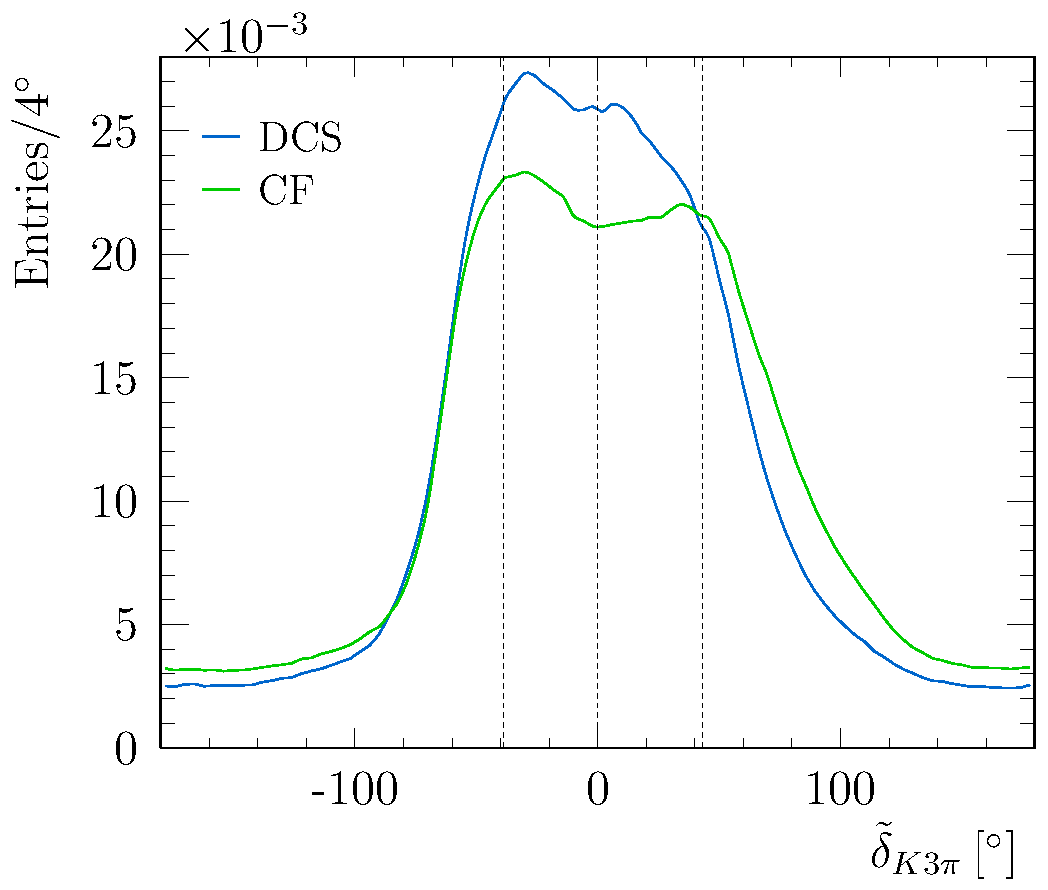
\includegraphics[width=0.45\textwidth]{Figures/K3pi_Binning_Scheme.pdf}
  \end{figure}
  \vspace{-0.5cm}
\end{frame}

\begin{frame}{$D\to K^-\pi^+\pi^-\pi^+$}
  \vspace{0.0cm}
  {\large And indeed, the coherence factor is greatly improved in bin $2$ and $3$!}
  \begin{figure}
    \centering
    \begin{subfigure}{0.5\textwidth}
      \centering
      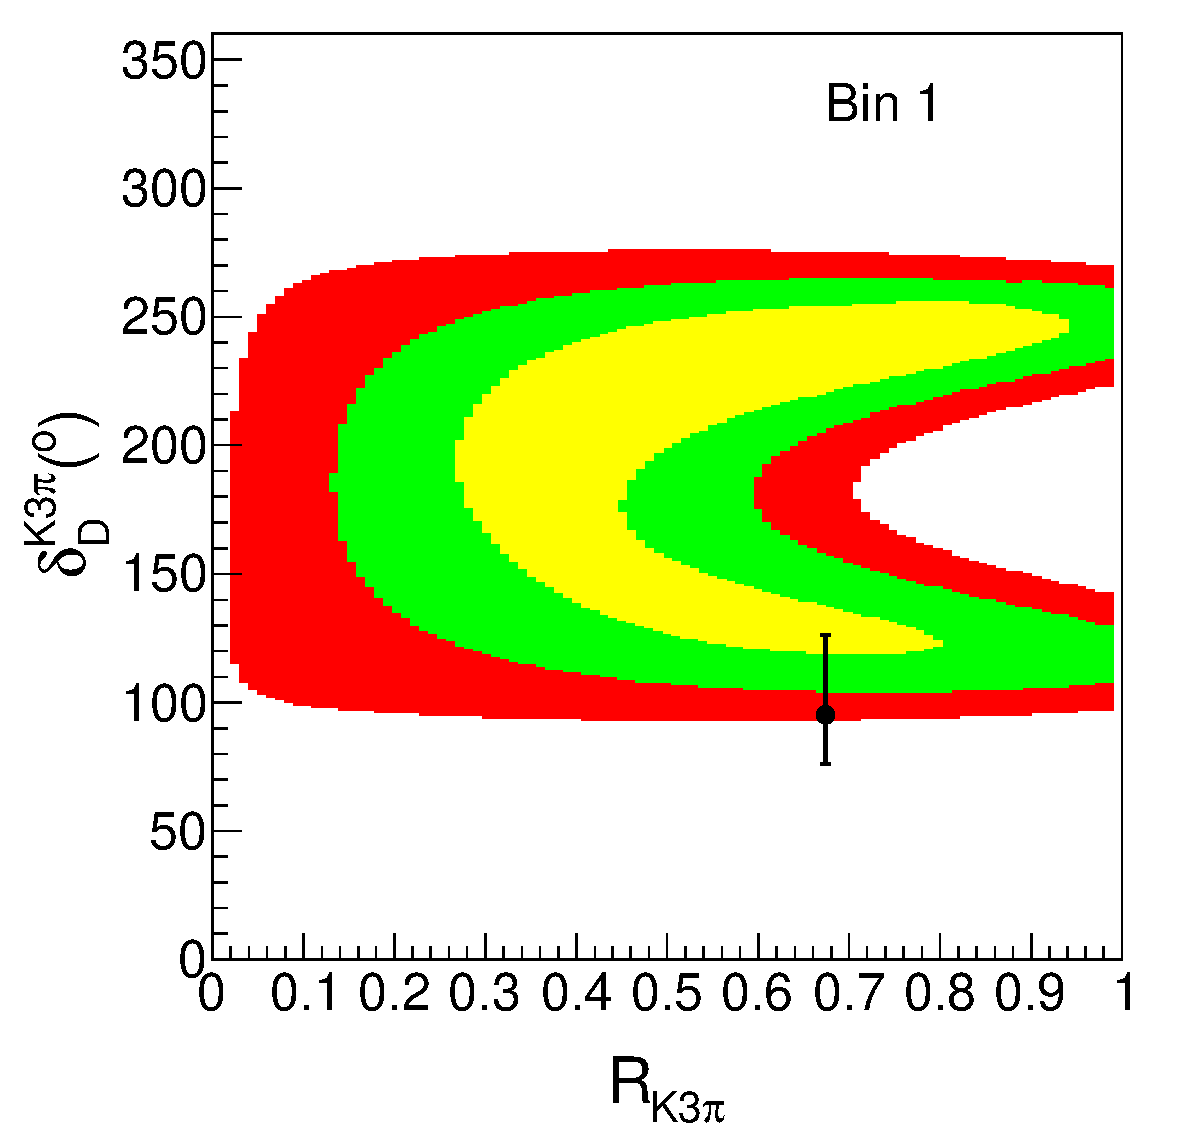
\includegraphics[height=3.0cm,width=3.5cm]{Figures/K3pi_Binned_Fit_Bin1.pdf}
    \end{subfigure}%
    \begin{subfigure}{0.5\textwidth}
      \centering
      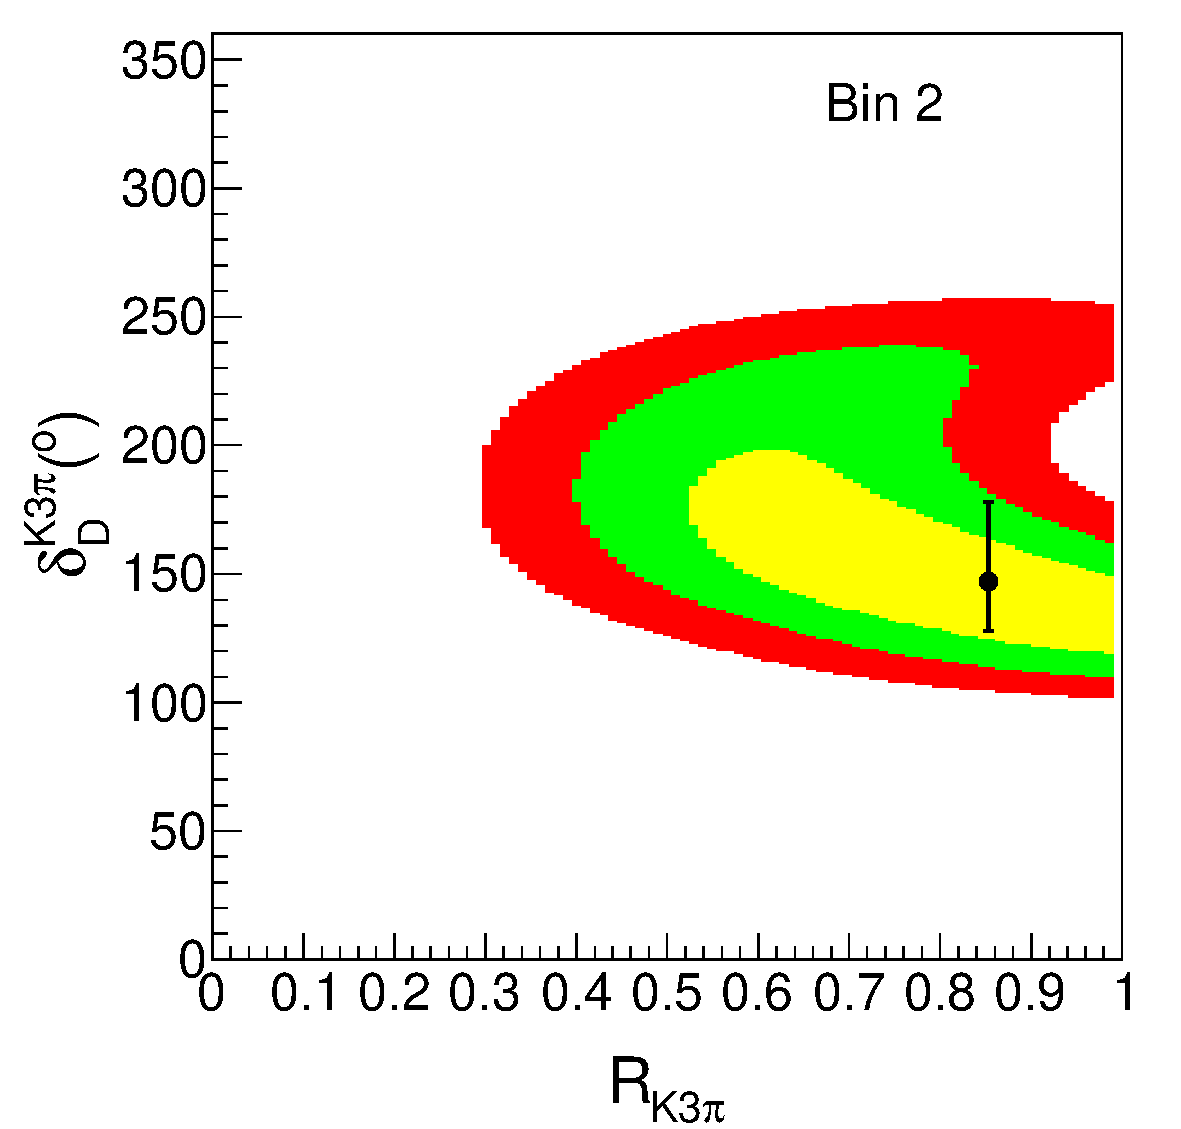
\includegraphics[height=3.0cm,width=3.5cm]{Figures/K3pi_Binned_Fit_Bin2.pdf}
    \end{subfigure}
    \begin{subfigure}{0.5\textwidth}
      \centering
      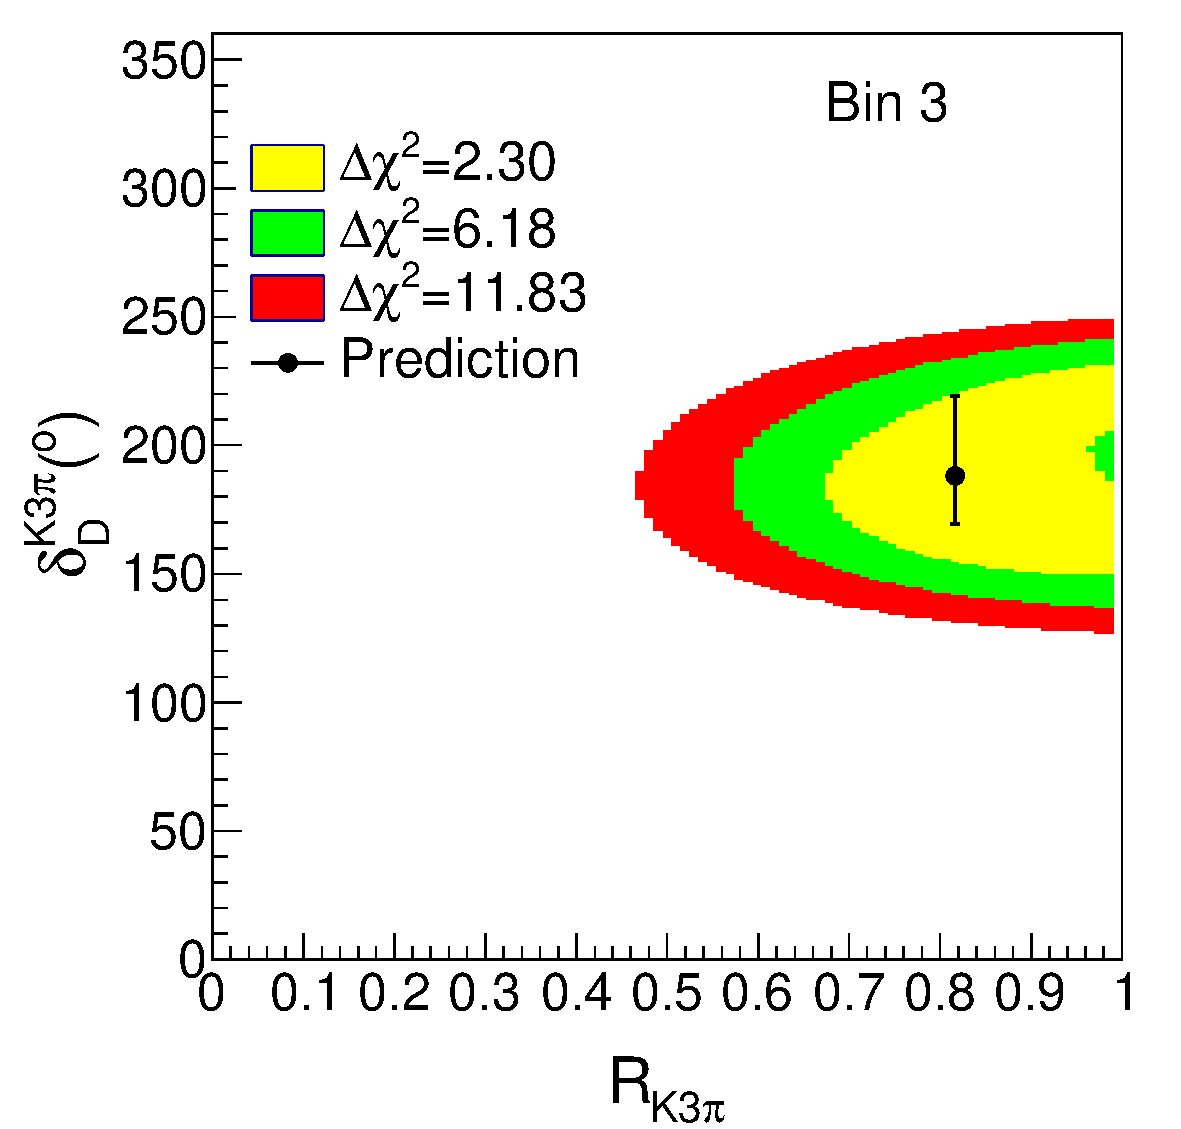
\includegraphics[height=3.0cm,width=3.5cm]{Figures/K3pi_Binned_Fit_Bin3.pdf}
    \end{subfigure}%
    \begin{subfigure}{0.5\textwidth}
      \centering
      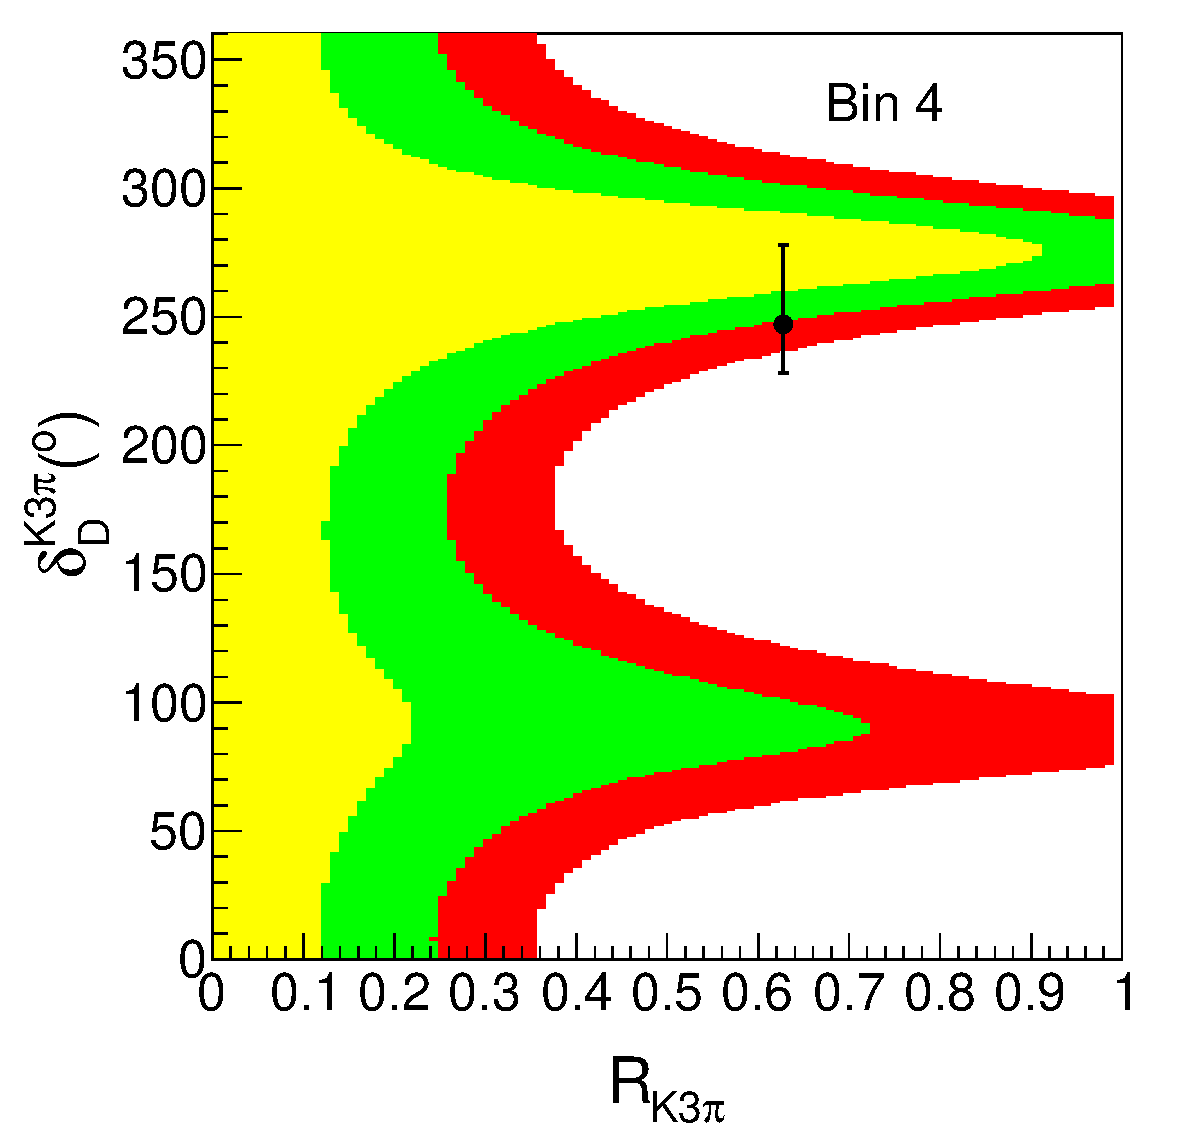
\includegraphics[height=3.0cm,width=3.5cm]{Figures/K3pi_Binned_Fit_Bin4.pdf}
    \end{subfigure}
    \caption*{Binned fit of $\delta_{K3\pi}$ and $R_{K3\pi}$.}
  \end{figure}
\end{frame}

\section{\texorpdfstring{$D\to K^+K^-\pi^+\pi^-$}{D2KKpipi}}
\begin{frame}{$D\to K^+K^-\pi^+\pi^-$}
\begin{tcolorbox}[enhanced,frame style image=blueshade_cropped.png,
  opacityback=0.75,opacitybacktitle=0.25,
  colback=blue!5!white,colframe=blue!75!black,
  title=\color{white}{\href{https://journals.aps.org/prd/abstract/10.1103/PhysRevD.107.032009}{\color{white}{Phys. Rev. D \textbf{107} 032009}}}]
  {\Large Measurement of the $C\!P$-even fraction of $D^0\to K^+K^-\pi^+\pi^-$}
\end{tcolorbox}
  What is measured:
  \begin{itemize}
    \item{Phase-space integrated strong-phase analysis of $D\to K^+K^-\pi^+\pi^-$}
  \end{itemize}
  Analysis strategy:
  \begin{itemize}
    \item{Uses a combination of $C\!P$ and multi-body tags}
    \item{Novel partially reconstructed technique to mitigate low efficiencies}
  \end{itemize}
  Significance:
  \begin{itemize}
    \item{First model-independent study of the $C\!P$ content of this decay}
  \end{itemize}
\end{frame}

\begin{frame}{$D\to K^+K^-\pi^+\pi^-$}
  \vspace{0.0cm}
  {\large This decay suffers from both low branching fraction and low efficiency, as seen in the double-tag fits}
  \begin{figure}
    \centering
    \begin{subfigure}{0.5\textwidth}
      \centering
      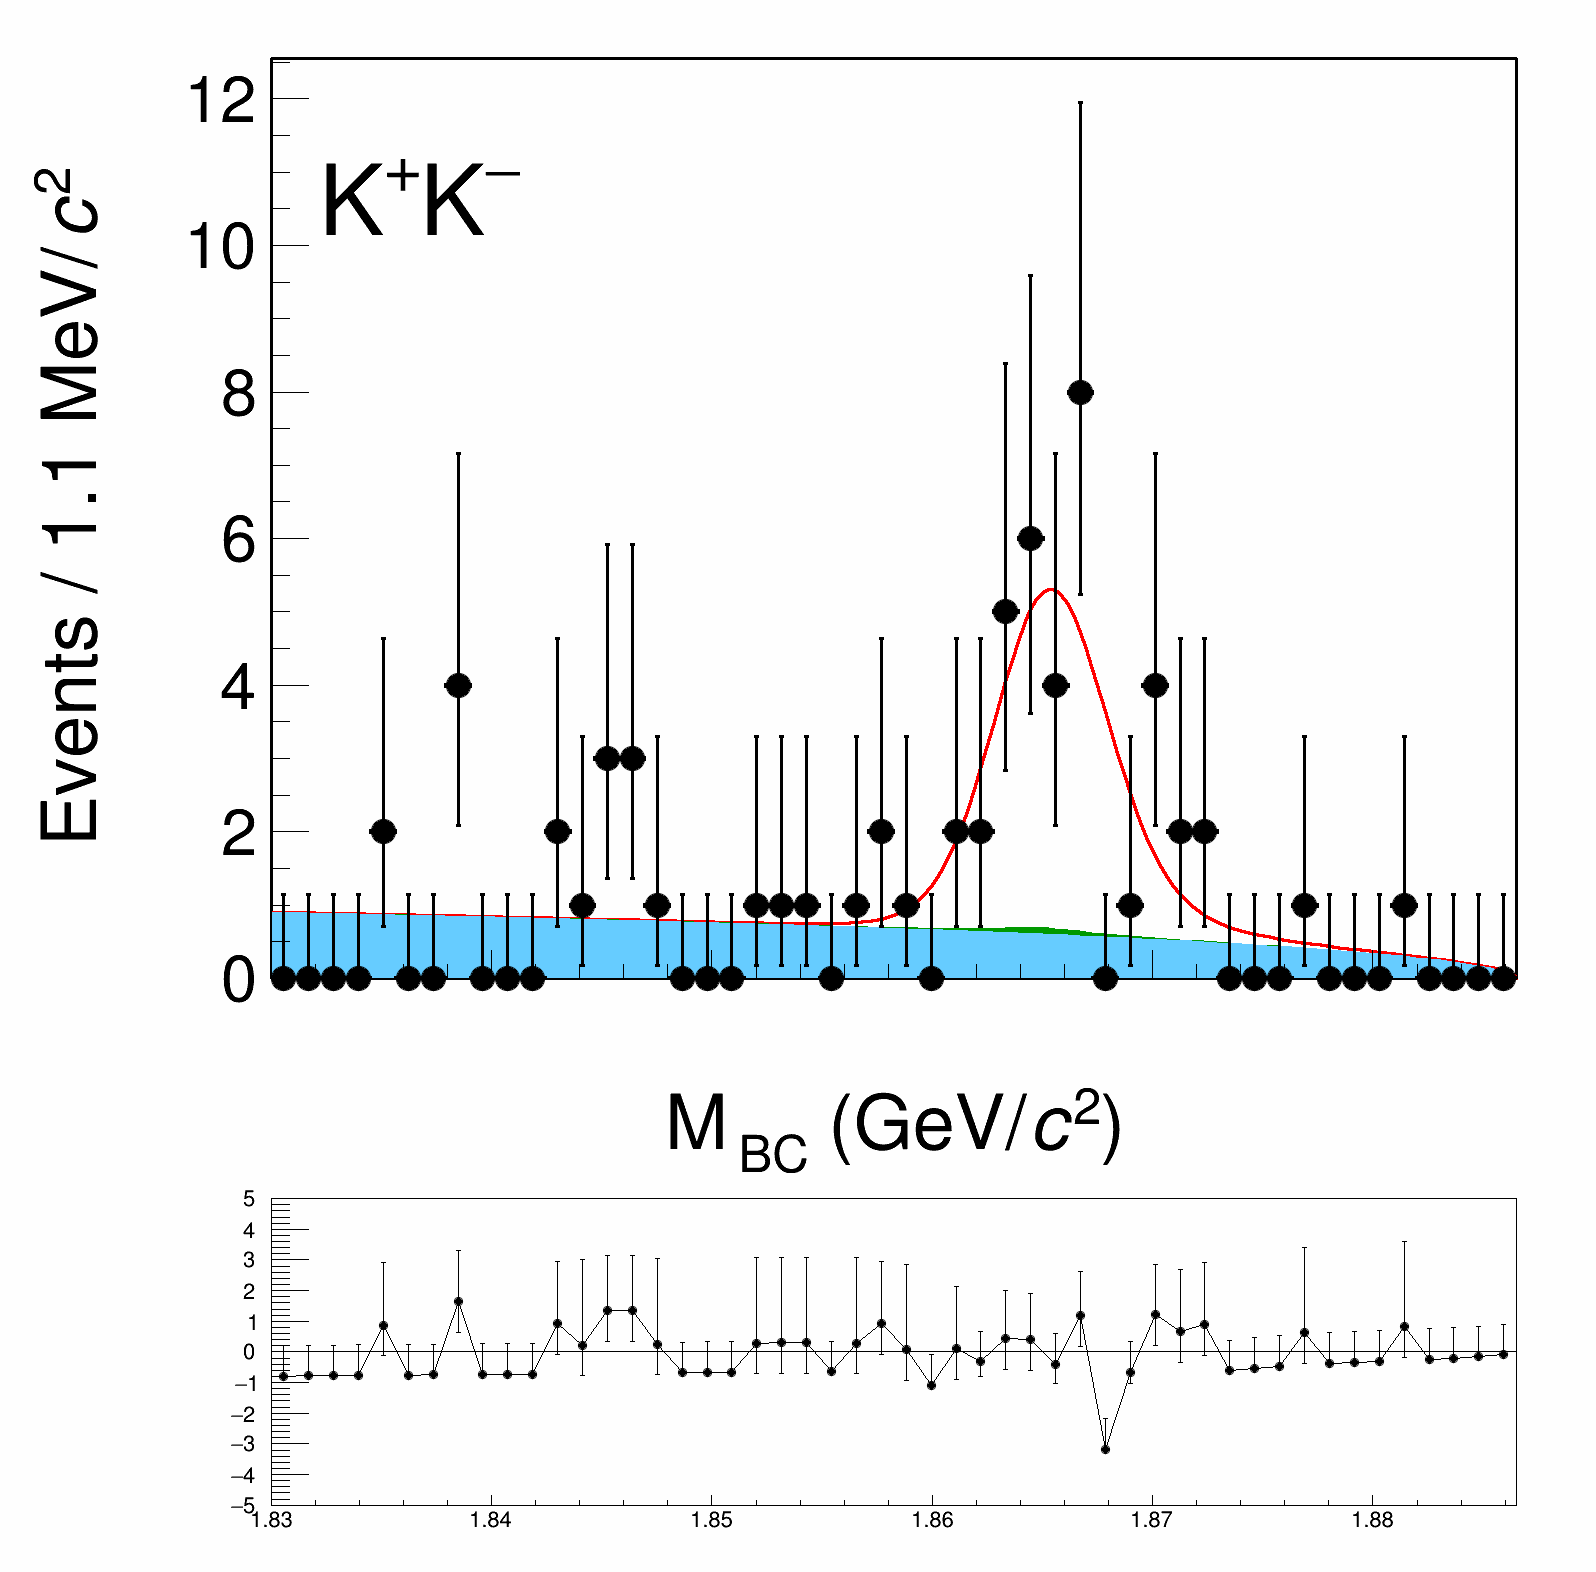
\includegraphics[height=4.0cm,trim={0 14.0cm 0 0},clip=true]{Figures/DoubleTagYield_DoubleTag_CP_KKpipi_vs_KK_SignalBin0.png}
    \end{subfigure}%
    \begin{subfigure}{0.5\textwidth}
      \centering
      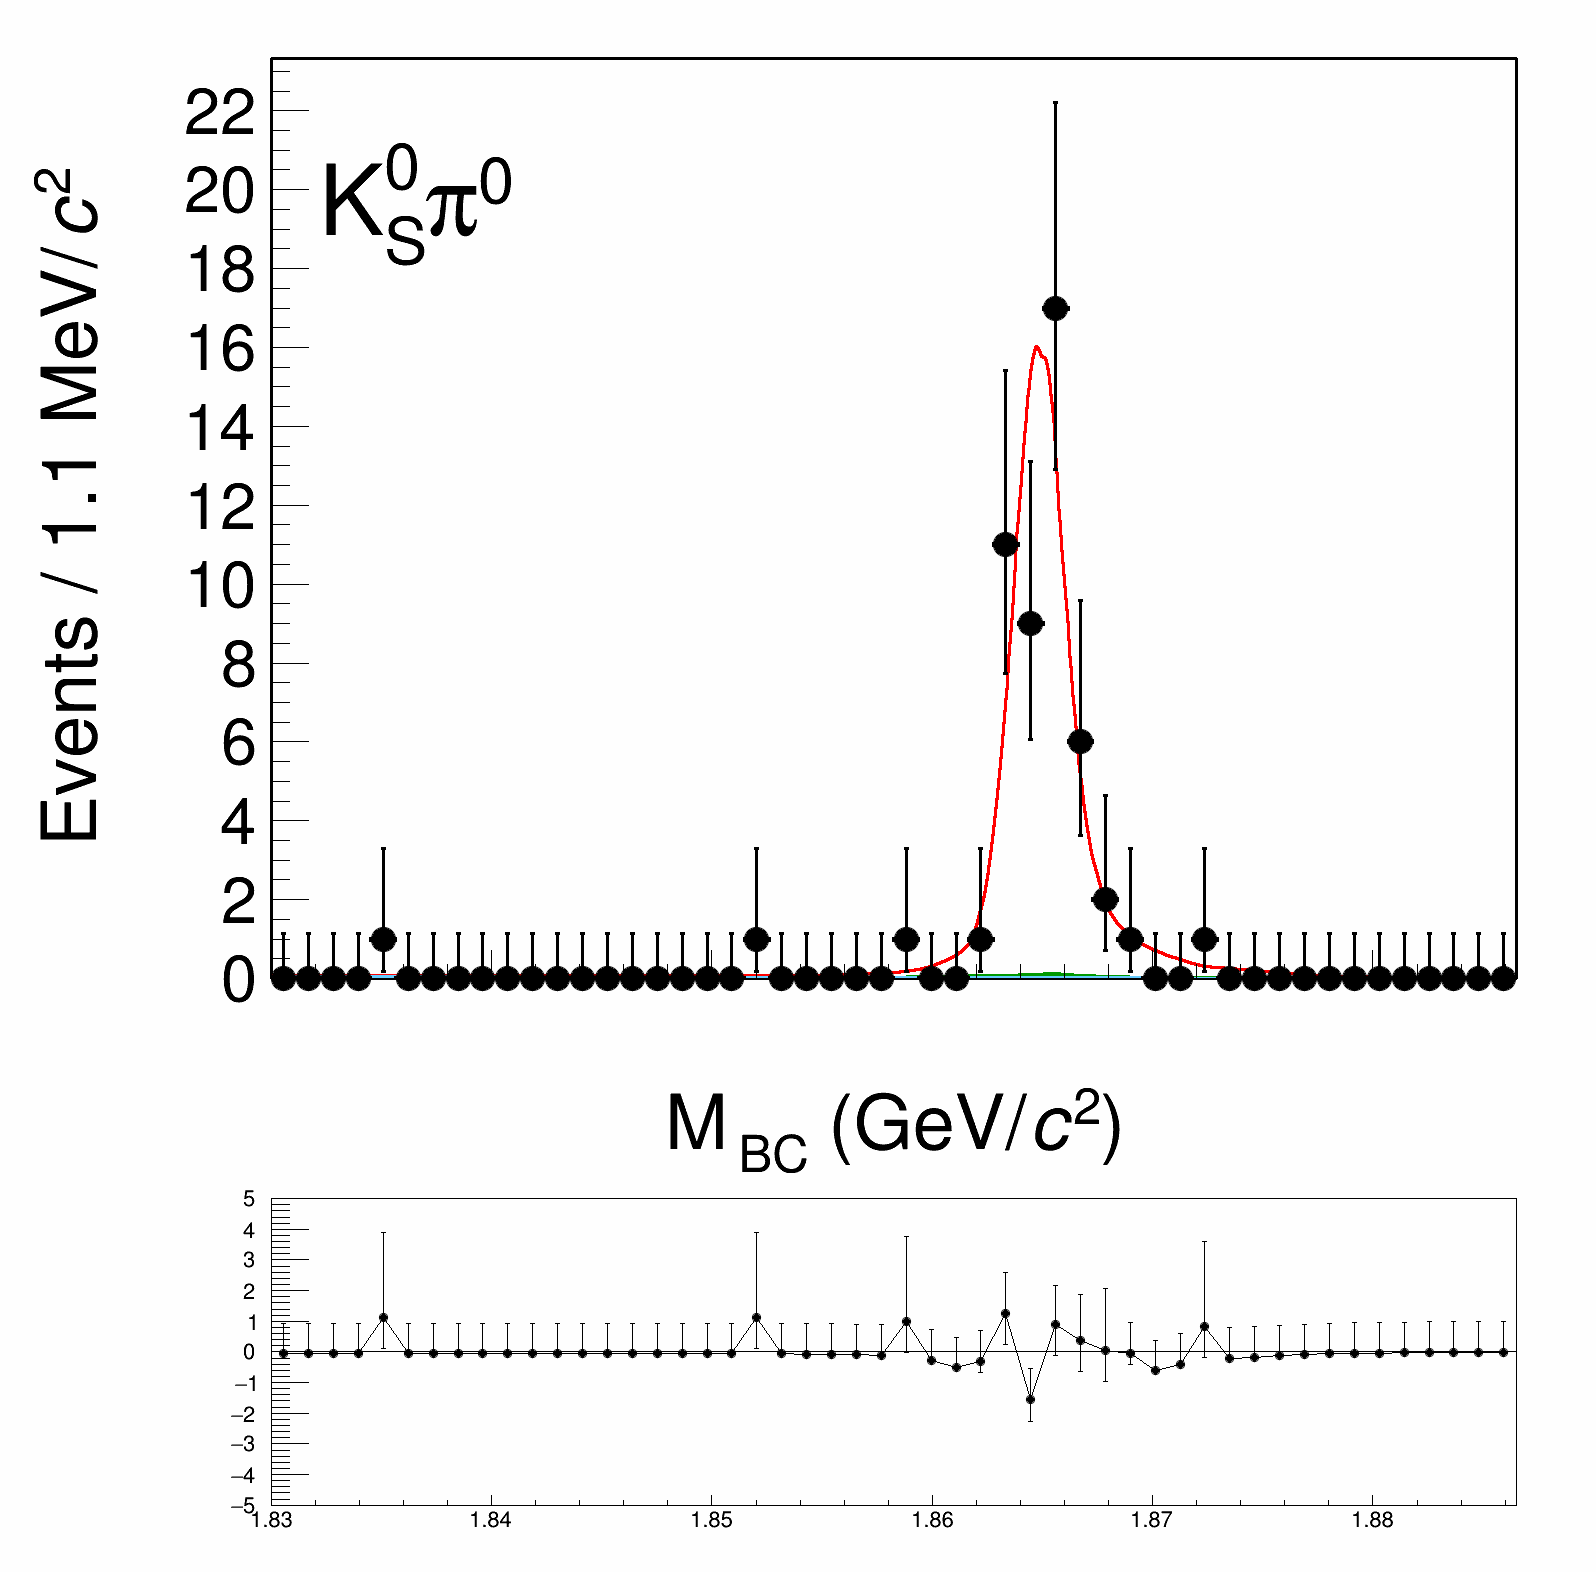
\includegraphics[height=4.0cm,trim={0 14.0cm 0 0},clip=true]{Figures/DoubleTagYield_DoubleTag_CP_KKpipi_vs_KSpi0_SignalBin0.png}
    \end{subfigure}
    \caption*{Double-tag fits of $K^+K^-\pi^+\pi^-$ vs (left) $K^+K^-$ and (right) $K_S^0\pi^0$.}
  \end{figure}
  {\large Clear quantum correlation: The yield of $K^+K^-\pi^+\pi^-$ vs $K^+K^-$ ($C\!P$-even) is suppressed, while that of $K_S^0\pi^0$ ($C\!P$-odd) is enhanced}
\end{frame}

\begin{frame}{$D\to K^+K^-\pi^+\pi^-$}
  \vspace{0.0cm}
  {\large The strong-phase information is parameterised in terms of the $C\!P$-even fraction $F_+$:}
  \vspace{-0.5cm}
  \begin{equation*}
    \frac{N^{\rm DT}}{N^{\rm ST}}\propto 1 \mp (2F_+ - 1)
  \end{equation*}
  \vspace{-0.5cm}
  \begin{figure}
    \centering
    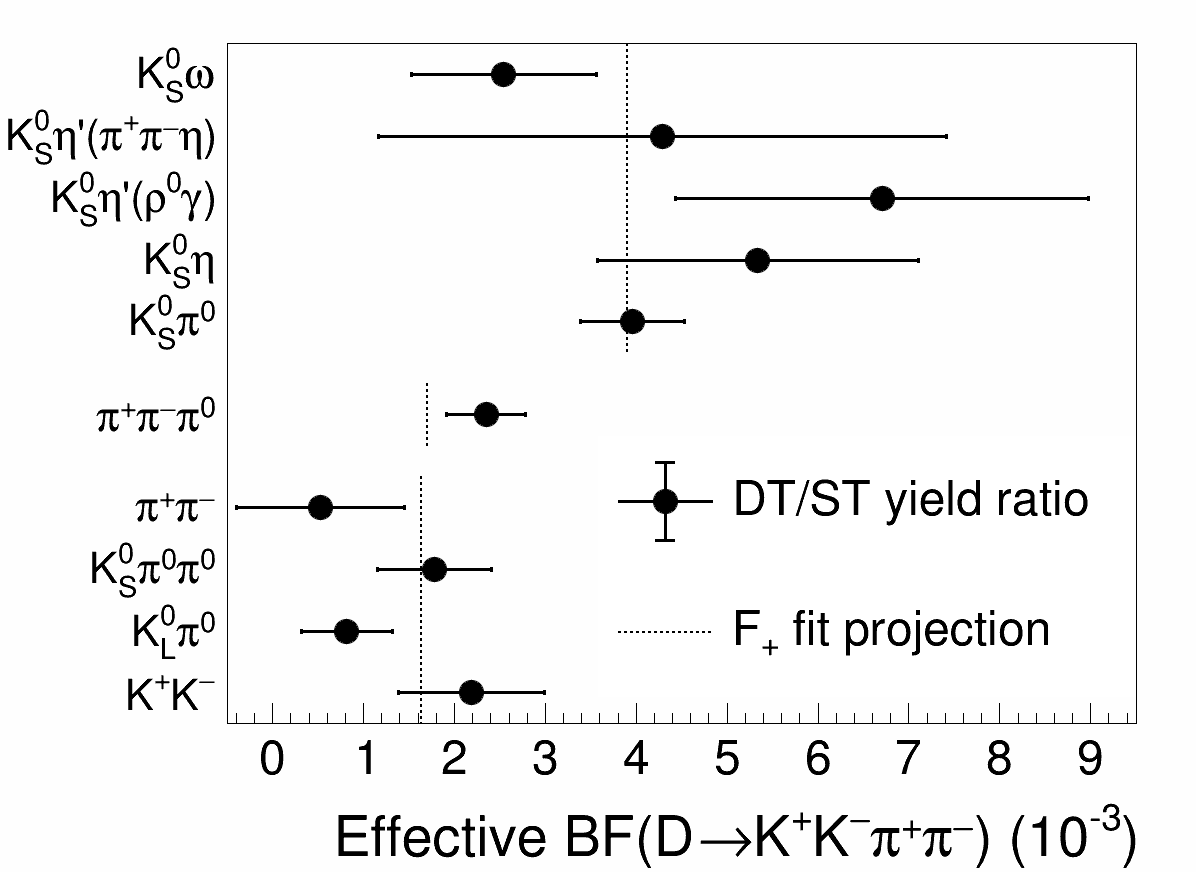
\includegraphics[width=0.55\textwidth]{Figures/CPeven_fraction_combination_CPtags.png}
    \caption*{Branching fractions of $D\to K^+K^-\pi^+\pi^-$ measured against $C\!P$-even/odd tags.}
  \end{figure}
  \vspace{-0.4cm}
  \begin{center}
    {\large Clearly, $D^0\to K^+K^-\pi^+\pi^-$ is predominantly \underline{$C\!P$-even}}
  \end{center}
\end{frame}

\begin{frame}{$D\to K^+K^-\pi^+\pi^-$}
  \begin{itemize}
    \item{To mitigate the low reconstruction efficiency, explore a novel partially reconstructed technique}
    \item{Poor low momentum kaon tracking efficiency $\implies$ \\Only reconstruct one kaon}
  \end{itemize}
  \begin{figure}
    \centering
    \begin{subfigure}{0.5\textwidth}
      \centering
      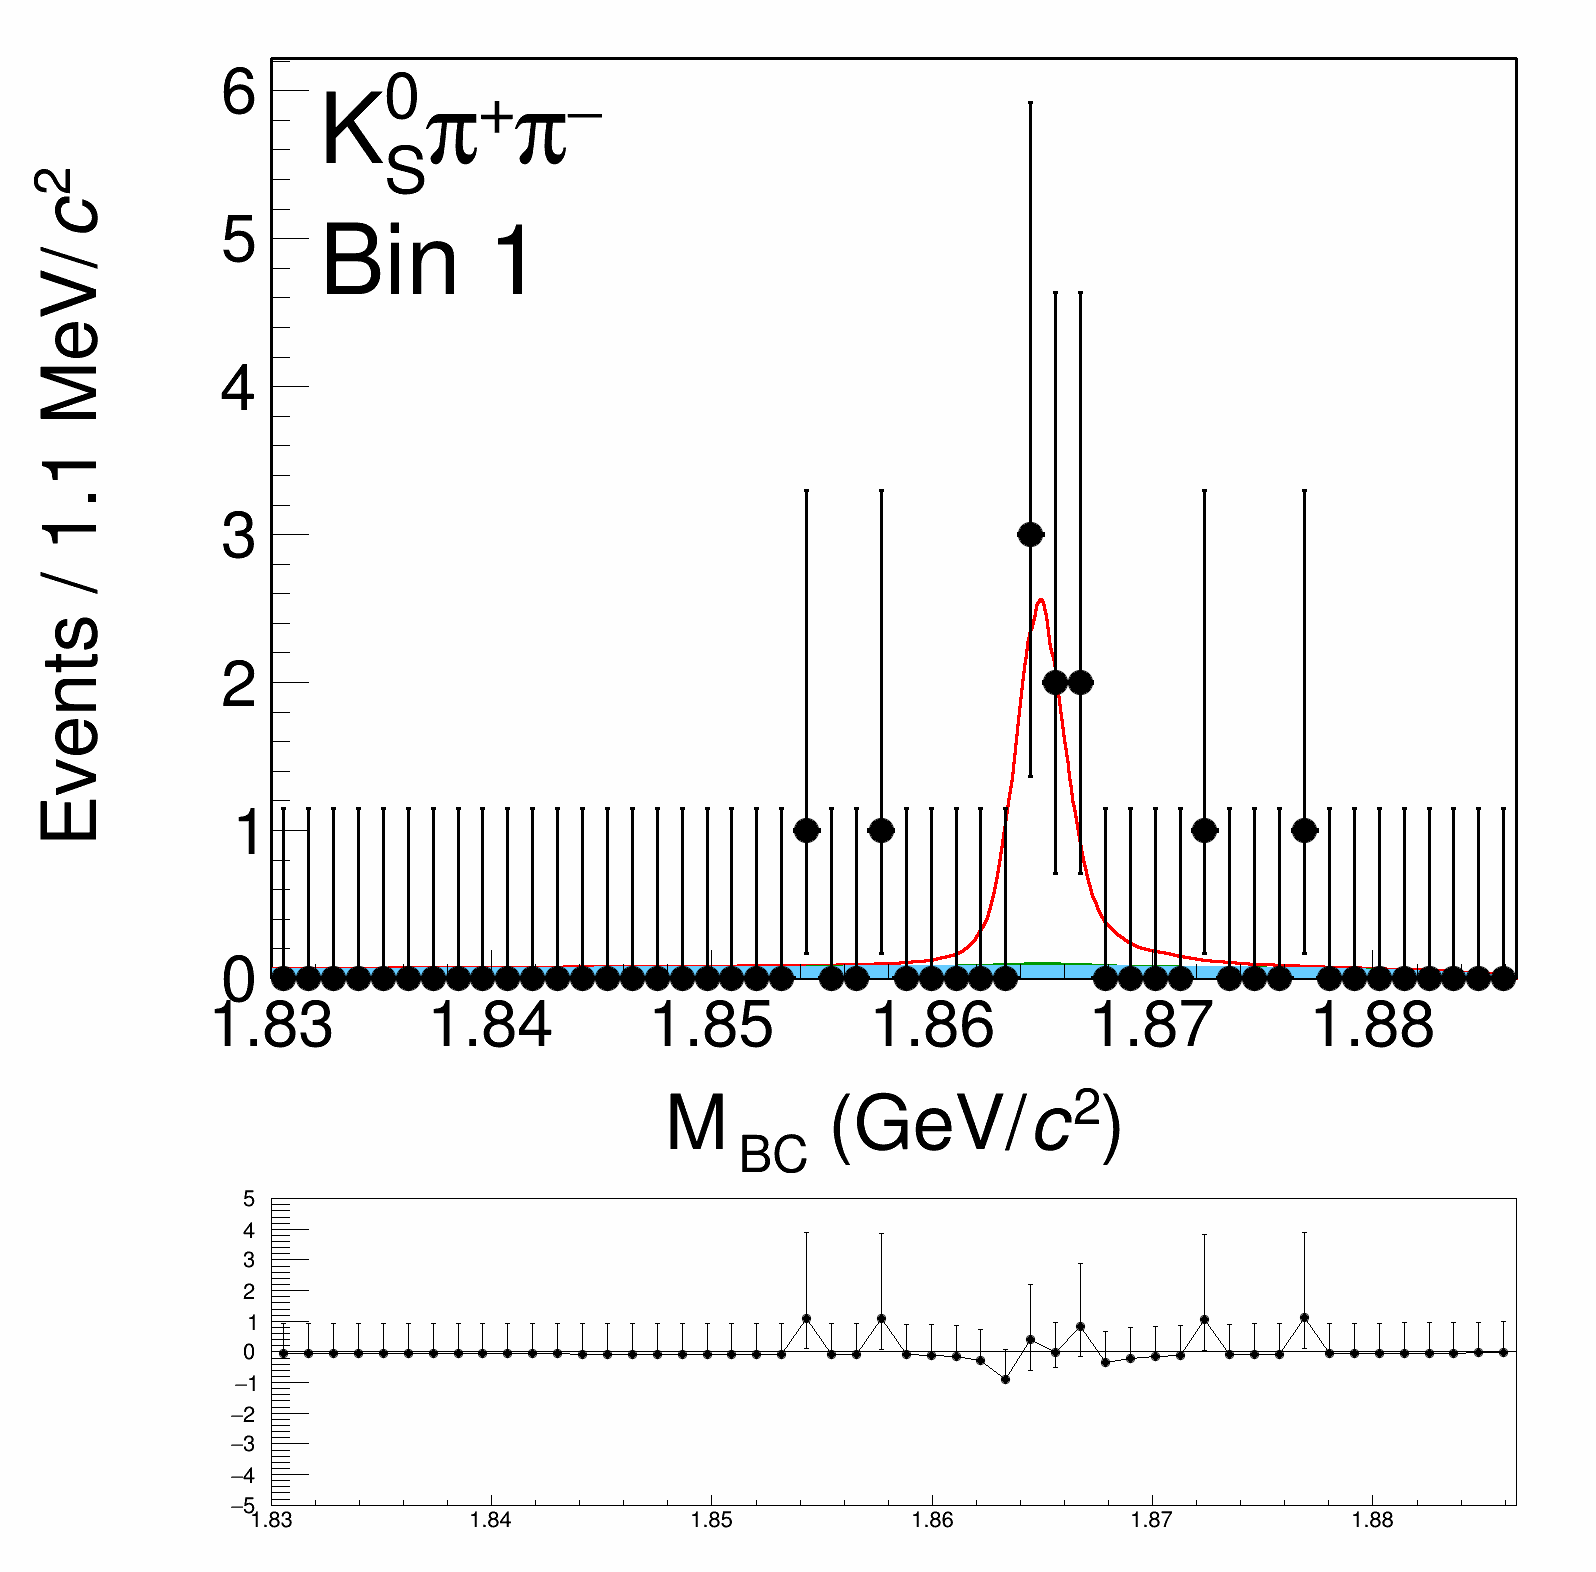
\includegraphics[height=4.0cm,trim={0 14.0cm 0 0},clip=true]{Figures/DoubleTagYield_DoubleTag_SCMB_KKpipi_vs_KSpipi_SignalBin0_TagBin1.png}
    \end{subfigure}%
    \begin{subfigure}{0.5\textwidth}
      \centering
      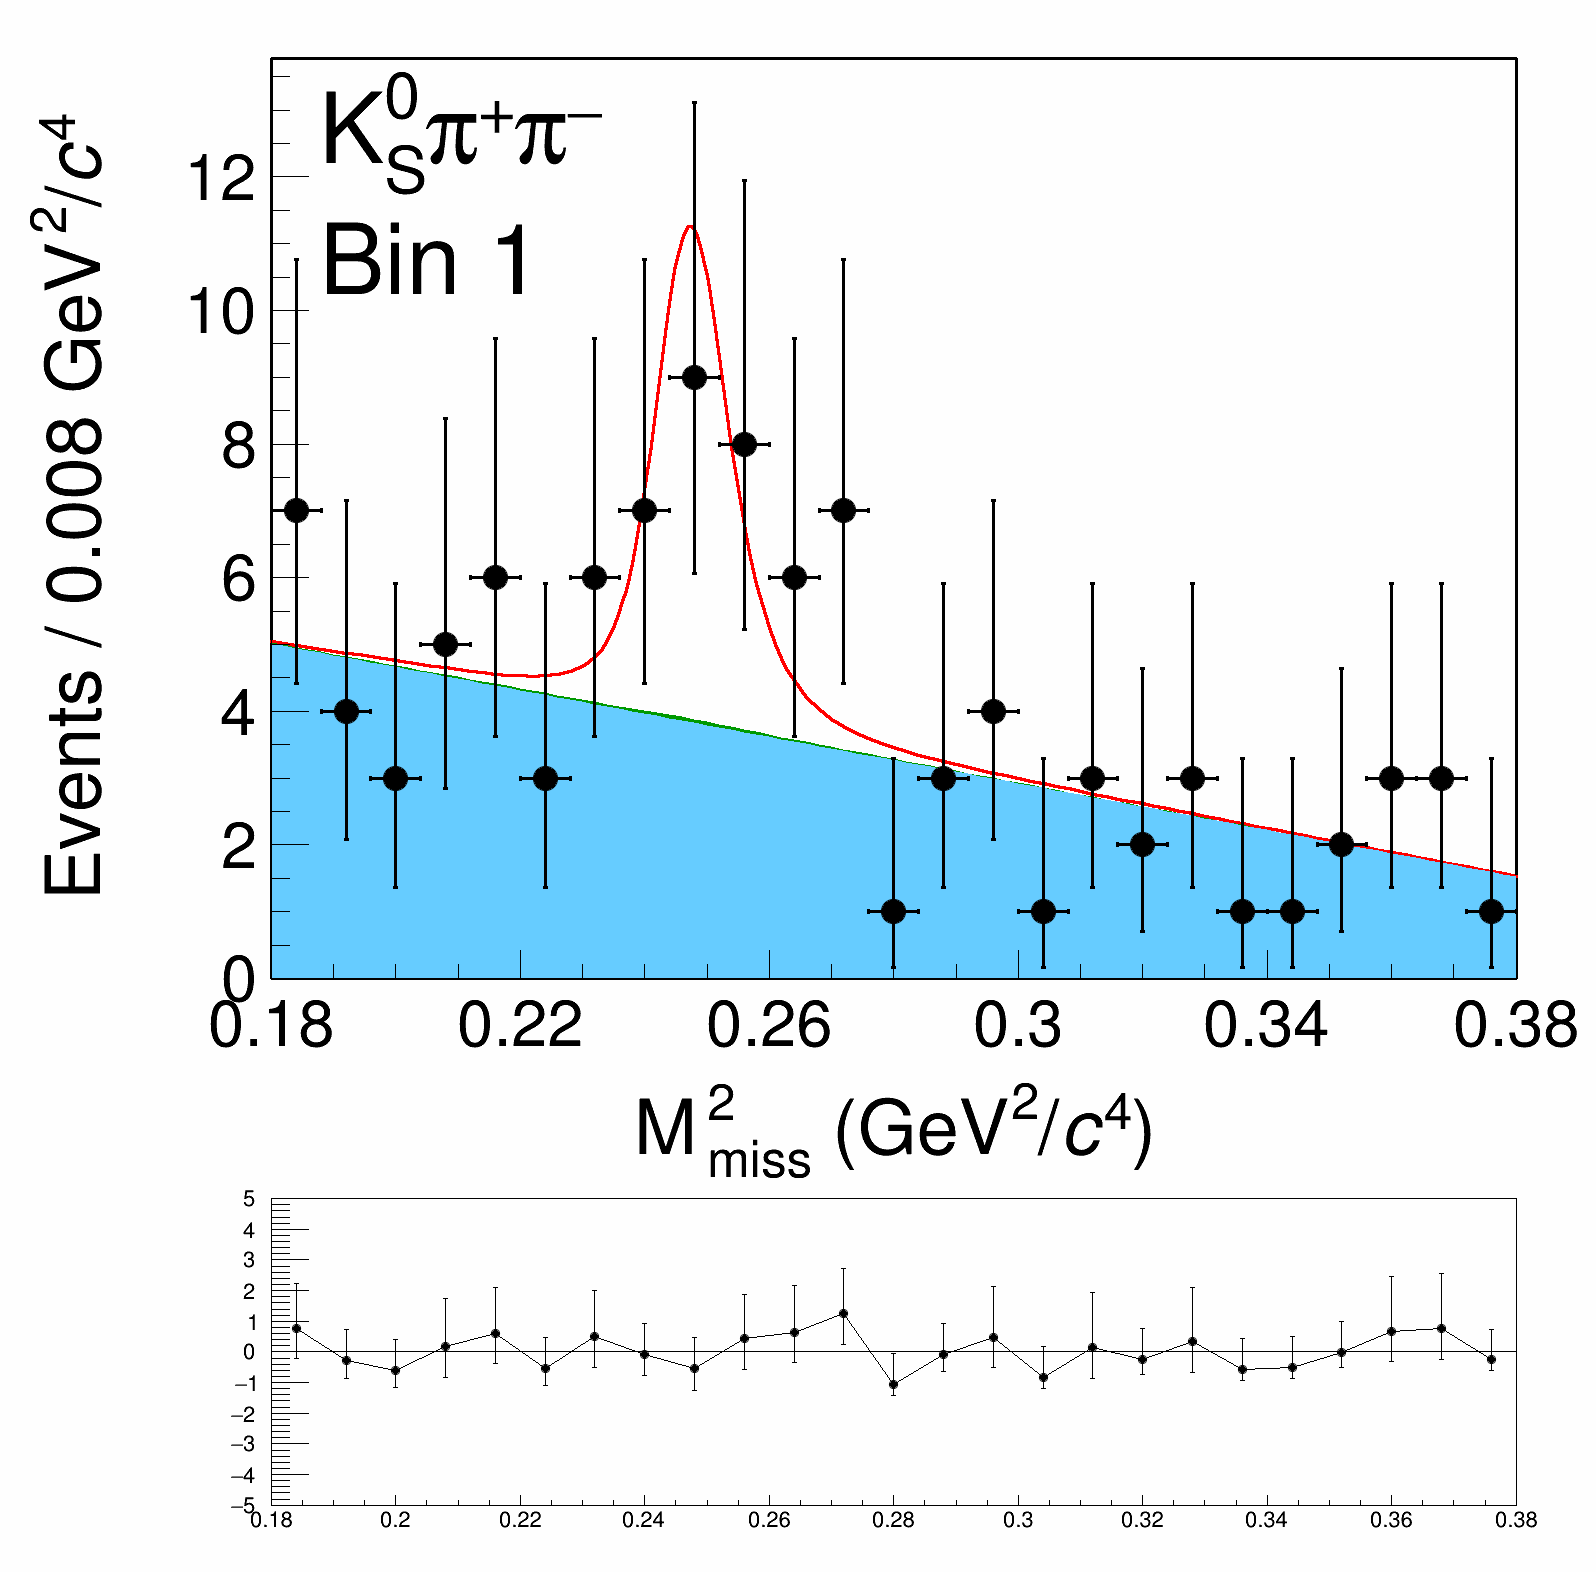
\includegraphics[height=4.0cm,trim={0 14.0cm 0 0},clip=true]{Figures/DoubleTagYield_DoubleTag_SCMB_KKpipi_vs_KSpipiPartReco_SignalBin0_TagBin1.png}
    \end{subfigure}
    \caption*{Fits of (left) fully and (right) partially reconstructed $K^+K^-\pi^+\pi^-$ vs $K_S^0\pi^+\pi^-$.}
  \end{figure}
\end{frame}

\begin{frame}{$D\to K^+K^-\pi^+\pi^-$}
  \vspace{0.0cm}
  {\large The multi-body tags $K_{S, L}^0\pi^+\pi^-$, which are split into phase-space bins, provide sensitivity to $F_+$}
  \begin{figure}
    \centering
    \begin{subfigure}{0.5\textwidth}
      \centering
      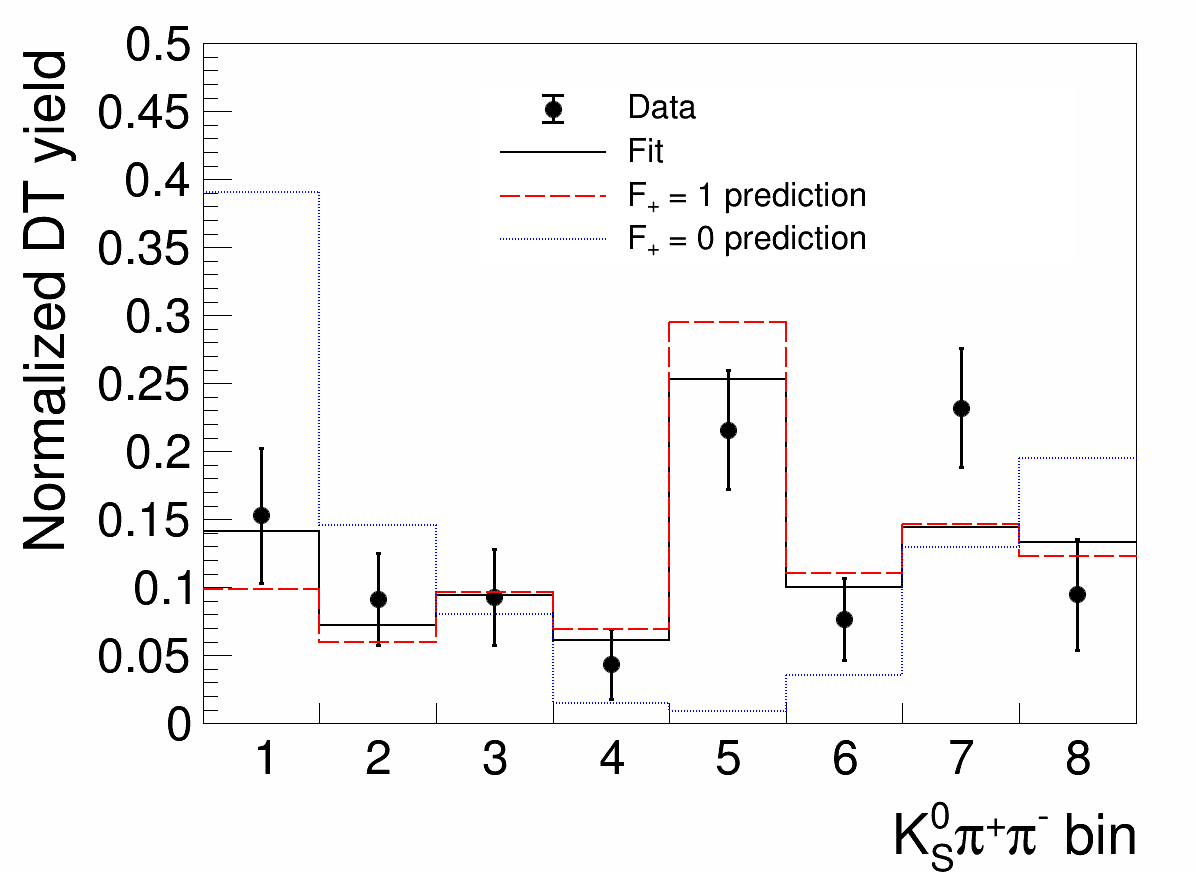
\includegraphics[height=4.0cm]{Figures/CPeven_fraction_combination_KSpipi.png}
    \end{subfigure}%
    \begin{subfigure}{0.5\textwidth}
      \centering
      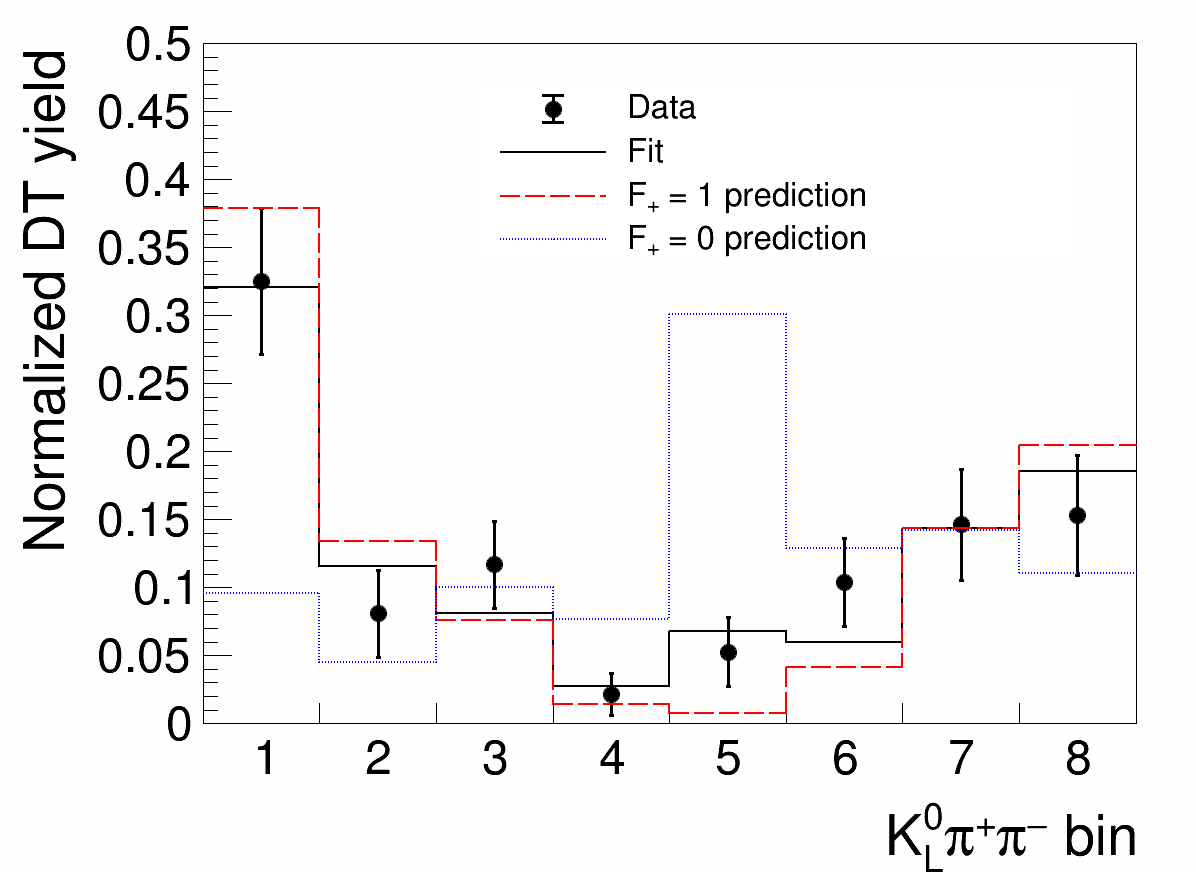
\includegraphics[height=4.0cm]{Figures/CPeven_fraction_combination_KLpipi.png}
    \end{subfigure}
    \caption*{Bin yields of $K^+K^-\pi^+\pi^-$ vs $K_{S, L}^0\pi^+\pi^-$.}
  \end{figure}
\end{frame}

\begin{frame}{$D\to K^+K^-\pi^+\pi^-$}
  \vspace{0.0cm}
  {\large Combining the $C\!P$ and $K_{S, L}^0\pi^+\pi^-$ tags:}
  \begin{align*}
    F_+ = 0.730 \pm 0.037 \pm 0.021 \\
  \end{align*}
  {\large This is not the end of the story:}
  \begin{enumerate}
    \setlength{\itemsep}{1.0em}
    \item{A phase-space binned analysis is ongoing}
    \item{The statistical precision will improve greatly with more data}
    \item{This fully charged mode will provide valuable inputs to $\gamma$ and charm mixing at LHCb and Belle II}
  \end{enumerate}
\end{frame}

\section{Summary and conclusion}
\begin{frame}{Summary and conclusion}
  \begin{enumerate}
    \setlength{\itemsep}{1.0em}
    \item{Many exciting measurements using quantum-correlated $D\bar{D}$ pairs have been performed, using the $\SI{3}{\per\femto\barn}$ dataset}
    \item{Previous analyses, such as $\delta_{K\pi}$, have been improved using more tags and more precise inputs}
    \item{BESIII is now exploring four-body decays, and many binned analyses are in the pipeline using the larger $\SI{8}{\per\femto\barn}$ dataset}
    \item{BESIII is expected to collect $\SI{20}{\per\femto\barn}$ of $\psi(3770)$ data by 2024}
    \begin{itemize}
      \item{Strong-phase measurements, which are currently statistics limited, will improve significantly in the next few years}
      \item{This unique dataset will be essential for providing inputs to the foreseen datasets at LHCb and Belle II}
    \end{itemize}
  \end{enumerate}
  \begin{center}
    \huge Thanks for listening!
  \end{center}
\end{frame}

\end{document}
